%  
%  in CH1 give an real life example at the begining as a BACKGROOUND
%  describe bacis concepts
%  and go into more details? obvious
%  
%  
%  
%  in CH2 active learning or web optimization
%  
%  
%  
\documentclass[12pt, a4paper, pdflatex, leqno]{report}
%  notitlepage - abstract on the same page
\usepackage{indentfirst} % indent frst paragraph of section
% \usepackage{fullpage}    % full A4 page
\usepackage[left=2.5cm, right=2.5cm, bottom=2.5cm, top=2.5cm]{geometry}

\usepackage{amsmath}
\usepackage{amsfonts}    % fancy maths font
\usepackage{mathrsfs}    % fancy maths font
\usepackage{dsfont}      % indocator finction
\usepackage{mathtools}

\usepackage[pdftex]{graphicx}
\usepackage{cite} % BiTeX
\usepackage{lipsum}
\newcommand{\ts}{\textsuperscript}
\usepackage[usenames,dvipsnames]{color}

% for multi figures
\usepackage{graphicx}
\usepackage{caption}
\usepackage{subcaption}

\usepackage[]{algorithm2e}

% \usepackage{polski}
% \usepackage[polish,english]{babel}
% \usepackage[utf8]{inputenc}
\usepackage[T1]{fontenc} % polsih

\usepackage{hyperref}

% Harvard citation
\usepackage[square]{natbib}

% argmax with commands
\newcommand{\argmax}{\operatornamewithlimits{argmax}}

% equality from definition | =^{\text{def}}
\newcommand{\myeq}{\stackrel{\mathclap{\normalfont\scriptsize\mbox{def}}}{=}}

% Code snippets
\usepackage{listings}
% \usepackage{color}


\definecolor{dkgreen}{rgb}{0,0.6,0}
\definecolor{gray}{rgb}{0.5,0.5,0.5}
\definecolor{mauve}{rgb}{0.58,0,0.82}

\lstset{frame=tb,
  language=R,
  aboveskip=3mm,
  belowskip=3mm,
  showstringspaces=false,
  columns=flexible,
  basicstyle={\small\ttfamily},
  numbers=none,
  numberstyle=\tiny\color{gray},
  keywordstyle=\color{blue},
  commentstyle=\color{dkgreen},
  stringstyle=\color{mauve},
  breaklines=true,
  breakatwhitespace=true
  tabsize=3
}
% END Code snippets

% $\backsim\ \sim\ \thicksim$

\newcommand{\HRule}{\rule{\linewidth}{0.5mm}}

\newenvironment{dedication}
  {\clearpage           % we want a new page
   \thispagestyle{empty}% no header and footer
   \vspace*{\stretch{1}}% some space at the top 
   \itshape             % the text is in italics
   % \raggedleft          % flush to the right margin
   \raggedright          % flush to the right margin
   \par\setlength{\leftskip}{0.3\textwidth}\noindent\ignorespaces
  }
  {\par % end the paragraph
   \vspace{\stretch{3}} % space at bottom is three times that at the top
   \clearpage           % finish off the page
  }

\begin{document}

\begin{titlepage}
\begin{center}
% Upper part of the page. The '~' is needed because \\
% only works if a paragraph has started.

\includegraphics[width=0.5\textwidth]{graphics/UOB-logo.png}~\\[2.5cm] % was 1cm

% \textsc{\LARGE University of Bristol}\\[1.5cm]

%\textsc{\Large Final year project}\\[0.5cm]

% \colorbox{magenta}{problem}

% Title
\HRule \\[0.4cm]
{ \huge \bfseries %\\[0.5cm]
	Comprehensive introduction to \emph{\textbf{Multi-armed bandits}}:\\[.5cm]
  \emph{Thompson Sampling}\\
  \&\\
  Active Learning in the bandits scenario\\[0.4cm] }
\HRule \\[1.5cm]

% Author and supervisor
\begin{minipage}{0.4\textwidth}
\begin{flushleft} \large
\emph{Author:}\\
Kacper B. \textsc{\textbf{Sokol}}
\end{flushleft}
\end{minipage}
\begin{minipage}{0.4\textwidth}
\begin{flushright} \large
\emph{Supervisor:} \\
Dr.~David \textsc{\textbf{Leslie}}
\end{flushright}
\end{minipage}

\let\thefootnote\relax\footnote{Level H/6 $|$ MATH 32200---20cp Project}

\vfill

% Bottom of the page
{\large \today}
\end{center}
\end{titlepage}



%Acknowledgment
\begin{center}Acknowledgement of Sources\\[2cm]\end{center}
For all ideas taken from other sources (books, articles, internet), the source of the ideas is mentioned in the main text and fully referenced at the end of the report.\\[0.5cm]
All material which is quoted essentially word-for-word from other sources is given in quotation marks and referenced.\\[.5cm]
Pictures and diagrams copied from the internet or other sources are labelled with a reference to the web page,book, article etc.\\[2cm]
Signed:\\[1cm]
Dated:~~~~~~~~~~~~\today

% \thispagestyle{empty}% no header and footer
\thispagestyle{empty}
\cleardoublepage
\pagestyle{plain}
\vfill



% \title{\emph{Multi-armed bandits} problem.\\
% 	Practical introduction to the problem for everyone.\\
% 	Real life application.}
% \author{Kacper Sokol\\University of Bristol, UK}
% \date{\today}
% \maketitle
% \begin{flushright}
% Supervised by:\\
% \textbf{David Leslie}
% \end{flushright}
% \begin{center}
% \line(1,0){250}
% \end{center}

\begin{abstract}
\thispagestyle{empty}% no header and footer
This dissertation covers two main topics: multi-armed bandits theory with extensive treatment of Thompson Sampling approach as well as application of MAB in active learning. The comprehensive introduction to the theory underlying multi-armed bandits is gradually developed to cover concepts necessary for understanding the basic bandits strategies. The later part of this dissertation presents first of its kind(as far as we know) application of Thompson Sampling inspired MAB algorithm to solve computer science task of learning in the environment of insufficient information.\\
Reader does not require any prior knowledge in this field, only basics of statistics and probability theory are necessary to smoothly follow the text.\\
\begin{center}
Keywords: \textbf{multi-armed, bandit, active, semi-supervised, learning, exploration, exploitation, Thompson Sampling}

\let\thefootnote\relax\footnote{\noindent This dissertation together with all figures and experiment source code is available as \texttt{GitHub} repository at: \url{https://github.com/So-Cool/MAB}.}

\end{center}
\end{abstract}

\begin{dedication}
I would like to thank my parents who provides me with any kind of support. For their guidance and advice which helps me to make the right choices throughout the life and fulfill my dreams.\newline

It would also be a painful journey without my supervisor Dr.~David~Leslie who always served me with an advice how to ``read'' and ``write'' all the maths and avoid unnecessary and overwhelming clutter in the books.\newline

Finally, big thanks to Iza and Kuba who often take care of my leisure time even though it always lacks.\\[2cm]


% \foreignlanguage{polish}{}
\begin{flushright}
Dzi\k{e}kuj\k{e} mamo,\\
dzi\k{e}kuj\k{e} Tomek.
\end{flushright}



% I was lost now I'm found
\textcolor{white}{found me!}



\end{dedication}


\newpage
\thispagestyle{empty}
\cleardoublepage
\pagestyle{plain}
\setcounter{page}{1}

\tableofcontents
% \newpage



\chapter{Introduction\label{chap:intro}}
The \emph{multi-armed bandits} problem has been rapidly developing field of statistics and probability theory since early 20\ts{th} century. With a vastly growing number of tasks that could be framed as a bandit scenario the field has become a topic of research for many scientists, economists not to mention companies looking for efficiency improvements and savings. All things considered, these problems can be solved with ease by finding a balance between \emph{exploration} and \emph{exploitation}.\\

Multi-armed bandits are a class of problems originated from a sequential allocation dilemma. They were defined during Second World War and quickly reached the fame of being too difficult to solve to become abandoned for decades. First general solution was constructed by John Gittins\ref{sec:gitind} in late 60's nevertheless, his work was overlooked for almost 20 years to become renown in the early 80's.~\citep{gittins+glazebrook+weber}

\noindent The main reference for this chapter is~\citep{berry+firstedt}.\\


\section{Background}
Many people consider statistics and probability as analyzing processes or data in various aspects---as a rather \emph{static} science. But what if the process of our interest is continuously developing while we want to discover it or it demands our interaction? Simple statistics or probability might not be able to handle such cases as good as bandits theory.\\

To begin with, lets consider \emph{fruit machine} as it is a first thing that comes to reader's mind after hearing about multi-armed bandits. Imagine a row of slot machines in front of you. Pulling an arm of each of these automaton will result in different outcome each with corresponding probability according to some unknown distribution. For the simplicity we will consider result as various reels combinations and we will assume that each automaton gives binary result: \emph{win} with probability $p$ and \emph{loose} with probability $p-1$. Without lost of any information, row of such machines can be transformed into only one automation but with multiples arms or buttons each corresponding to single machine in a mentioned row.\\

The natural example that follows binary bandits is a row of coins, where some of them may be unfair. In presented scenario each coin corresponds to an \emph{Arm} of a bandit and tossing one of them for several times can be considered as realization of a Bernoulli process with unknown parameters.\\
If a player is rewarded when the outcome of a trial is \textbf{H}ead then the goal is to find the coin which has bias with maximum probability of \textbf{H} and play it forever.\\

If a gambler does not want to loose all possessed money really quick it would be probably a good idea to have some kind of strategy that maximizes chances of winning. It is assumed that the gambler is for the first time in a given casino so any prior information regarding expected return from each arm is assumed to be unknown. Initially random arm is chosen as all of them ``look the same''. On contrary, during the second turn selecting \emph{optimal} arm to be played becomes a serious dilemma that you might have not yet realized. The gambler faces a choice between already pulled arm with sample expected return that is known and any other arm which for now on remain a mystery as there is no information about potential reward.\\
If gambler decides to take advantage of already known arm and pull it again we call this action \emph{exploitation}---that is taking advantage of already checked possibilities. On the other hand, taking a risk and choosing one of the unknown arms will result in gathering some more information about the system what is usually said to be \emph{exploration} step.\\


\section{Applications} % emphasized underlying
Multi-armed bandits are not just a theory that one reads from a book and try to memorize; they extends to many real life applications. This section is devoted to simple case study in which it seems natural to use ``bandit approach''. Applications are versatile ranging from drug testing and maximizing income from web advertisement through semi-supervised machine learning in modern computer science as well as time and budget management of research projects.\\

To begin with, imagine a hospital testing two new medicines for a certain disease. Patients are queuing up to receive a treatment. Assuming that doctor cannot refuse to treat anyone, each person suffering from a disease(each \emph{play}) can be given two possible drugs(two \emph{arms}). The key assumption here is that the effect of chosen action occur immediately, in other words treated person either stays sick or is cured(immediate \emph{payoff}). The goal of a doctor is to maximize the number of healed people. This model defines two-armed bandit.\\

The second mentioned approach is nowadays widely incorporated by companies such as Google~\citep{AYPSze12, ASMB:ASMB874}, LinkedIn~\citep{Tang:2013:AAF:2505515.2514700}, Microsoft~\citep{graepel2010web}, Yahoo~\citep{Li:2010:CAP:1772690.1772758} to their services. Research groups of these companies are using bandits algorithms to choose the best website layout and advertisements locations to increase click-through rate(CTR)\footnote{Measure of success of an on-line advertising campaign.}, improve recommendation systems or enhance performance of semi-supervised and active learning algorithms in the field of machine learning.\\

The bandit theory also plays a key role in experiment allocation with restricted resources like time and budget~\citep{gittins+glazebrook+weber}. While considering bandit's \emph{arms} as research projects pending to be conducted with limited amount scientist, time or funding the goal is to maximize the number of accomplished tasks(\emph{payoff}) before distributing the money among them.\\

With all presented above scenarios barely scratching the tip of the iceberg we are now focusing on foundations of multi-armed bandits theory that one needs to precisely describe the processes happening ``behind the scene''.\\
We begin with introducing the reader with necessary notation and nomenclature. Then we are moving to basic process description.


\section{Terminology}
Statistical decision theory defines ``simple'' multi-armed bandit as a sequential selection from $N \geq 2$ stochastic processes---generally called \emph{arms}, where both time and processes may be discrete or continuous. The goal is typically to recover unknown parameters that characterize stochastic processes the \emph{arms} to maximize expected \emph{payoff}.\\

It is handy to be familiar with most common terms used to describe multi-armed bandit in papers and books. The basic concepts are:
\begin{description}
\item[Multi-armed bandit ($N$)]---a ``device'' with $N \geq 2$ possible choices of action(\emph{arms}).
\item[Agent]---a person who decides which \emph{arm} to pull based on chosen \emph{strategy} $\tau$.
\item[Strategy ($\tau$)]---tells the \emph{agent} which \emph{arm} to pull at given stage of the \emph{game}. A strategy is \emph{optimal} if it yields maximal expected \emph{payoff}.
\item[Arm]---one of $N$ actions that may be taken by the \emph{agent}. An \emph{arm} is \emph{optimal} if it is the best selection when following some \emph{optimal} strategy.
\item[Play]---an \emph{arm} pulled at stage $m$ of the \emph{game} (i.e.\ one turn).
\item[Game]---a sequence of \emph{arms} pulled based on chosen \emph{strategy} $\tau$.
\item[Payoff]---a return of a game such as \emph{win--loose} or \emph{amount} of money gained.
\item[Discount series]---factors that define how valuable is each of \emph{payoffs}. For example only first $m$ outcomes may count and all the rest is neglected or the longer the \emph{game} is played the less particular outcome counts toward overall expected \emph{payoff}.
\end{description}


\section{General assumptions}
Two fundamental assumptions to vast majority of bandit problems regard benefits from selecting an arm, namely:
\begin{itemize}
\item immediate \emph{Payoff} i.e.\ \emph{agent} knows the result of taken action immediately,
\item information gathered after a \emph{play} can be used to modify chosen \emph{strategy}.
\end{itemize}
Moreover in some cases we may restrict the memory of an \emph{agent} to last $s$ outcomes. Therefore, selected \emph{strategy} $\tau$ can relay on up to $s$ previous \emph{plays}. These bandits approaches are called \emph{finite memory}.\\
Majority of this dissertation assumes that \emph{arms} are independent. If this setting changes it will be clearly stated.


\section{Discount Sequence}
To specify the rules governing the ``significance'' of outcome from a single play at stage $m$ the \emph{discount sequence} is introduced. It is a vector $\mathbf{A}$ of specified length, which can also be infinite.
$$
\mathbf{A} = \left( \alpha_1, \alpha_2, \alpha_3, ... \right)
$$
When an \emph{arm} is selected the discount sequence is modified by left shift:
$$
\left( \alpha_1, \alpha_2, \alpha_3, ... \right)
\rightarrow
\left( \alpha_2, \alpha_3, \alpha_4, ... \right) \text{ .}
$$

\subsection{Most common sequences}
There are many different discount sequences used with multi-armed bandits each with numerous assumptions. In the literature only two of them are described in great detail and both are presented below.

\subsubsection{Uniform sequence}
This discount sequence is most commonly used when a player wants to maximize the payoff of the first $h$ outcomes.
The $h$-horizon uniform discount sequence is defined as:
$$
 \alpha_i =
  \begin{cases}
   1 & \text{for } i \leq n \\
   0 & \text{for } i > n \text{ ,}
  \end{cases}
$$
leading to:
$$
  \mathbf{A} = ( \underbrace{ 1, 1, 1, ..., 1}_{h\text{ elements}}, 0, 0, 0, ... ) \text{ .}
$$

After \emph{arm} selection the horizon of discount sequence is decreased by $1$.


\subsubsection{Geometric sequence}
The geometric discount sequence is expressed with components $\alpha_i = a^{i-1}$ for some $a \in ( 0, 1 )$ resulting in:
$$
\mathbf{A} = \left( a^0, a^1, a^2, ... \right) \text{ ,}
$$
where $\alpha_1 = a^0$ is always equal to $1$. The characteristic feature of this series is that after \emph{arm} selection the discount sequence is still proportional to the original sequence.\\

It can also be shown that when the discounting is geometric, a bandit problem involving $k$ independent arms can be solved by solving $k$ different two-armed bandits, each involving one known and one unknown arm.\\[2cm]



In case of both sequences the decision problem and optimal strategy is unchanged if a discount series is multiplied by some constant. Furthermore, the geometric sequence is effectively the same throughout the \emph{game}.


\subsubsection{Mixtures of uniform sequences}
If we consider Bernoulli trials(with success worth $1$) of a clinical test the experiment can terminate with positive probability $\nu_m$ at any stage $m$ as we do not know the exact number of incoming patients. In such cases we may form a discount sequence where factor at given stage is the probability that the experiment has not been terminated so far, $\alpha_m = \sum_{i=m}^\infty \nu_i$. Clearly discount series that arises in presented scenario is a mixture of uniforms. This case is identical to deterministic sequence---an average of uniforms weighted by the $\nu_m$'s.\\
An example my be a $\gamma$ probability of terminating at each stage therefore, the factor at each reached stage is: $\nu_m = (1-\gamma)\gamma^{m-1}, m=1,2,3,...$, leading to geometric discount sequence.

\subsubsection{Random discounting}
The random discounting is more complex. In mixture of uniforms we get no advantage conditioning on the past: as long as we get $1$ the process continues and there is no possibility that previous factors were $0$; once we get $0$ the process is no more of interest. In general, with random discount sequence we are only provided with some prior probability distribution over the space of all possible discount sequences.\\

\subsubsection{Observable and non-observable sequences}
Sometimes the discount sequence cannot be observed: it is either blended with a reward as a single value or it is not given to us together with the reward. In such cases we need to estimate it. Like in the random scenario, given the distribution over all possible discount sequences we can estimate it by: $\hat{\alpha}_m = \mathbb{E}(\alpha_m | \text{``probability distribution over all discount sequences''})$.\\

We say that a discount sequence is observable if together with a reward we get a value of discount factor at given stage. This cases may be harder to solve as with random sequences we cannot replace them with a non-random sequences without significantly altering the problem.\\
In presented scenarios strategies tend to depend on deterministic, observable discount factors.\\

\subsubsection{Real-time sequences}
In real time sequences the intervals between events are random therefore directly influence decision making process. To visualize this scenario we consider clinical trial with patients arriving in random time intervals. In such cases we usually use discount sequence described by: $A = ( \exp(-\beta t_1), \exp(-\beta t_2), \exp(-\beta t_3),... )$, where $\beta$ is weight coefficient and $t_i$ are known arrival times.\\
more complicated situation for real-time discounting can be described as:
$$
  \alpha_t =
    \begin{cases}
      1 & \text{for } t \in [0,1] \text{ ,} \\
      0 & \text{for } t \in [1,\infty) \text{ .}
    \end{cases}
$$
Such sequence can express interest in maximizing the response of patients arriving in first unit interval. It is worth noting that the action choice may be significantly different if the first event occurs at time $0.01$ then if it would occur at time $0.99$; generally, risky arm could be appropriate in first case and mean maximizing action can be a good choice in second case.\\

\subsubsection{Non-monotone sequences}
Majority of discount sequences considered in literature are monotone increasing or decreasing. This fact is motivated by real life applications where our interest in process decreases---the player is interested in  quick reward---or increases---the player is interested in high reward in the future by first learning about environment.\\
The most popular and one of a few non-monotone sequences are defined by: $\alpha_n = 1$ and $\alpha_m = 0$ for $m \neq n$. This structure of discount sequence indicate that the first $n-1$ stages are played for sole purpose of obtaining information to make the best possible choice at stage $n$ and all the other rounds do not matter.\\


\section{Bandits settings}
Multi-armed bandit setting can be used to solve variety of problems. The most common settings have been discussed in chapter~\ref{chap:intro}; nevertheless, some non-trivial environments are also used and presented below.\\
\subsubsection{Real time, random bandits}
Real time, random bandits are usually present when decision needs to be made for event of given class or assigned to particular problem that occur in non-deterministic intervals of time and information of the event can only be acquired during its occurrence. Such scenarios can be similar to ones described in \emph{Random discounting} section.\\
\subsubsection{Information gathering}
One of scenarios where multi-armed bandits are also used is to gather information about available choices. If such learning needs to be done in efficient manner MAB is often a good choice. An example presented in \emph{non-monotone} section, where a number of rounds at the beginning was used to learn some information about the environment is one of them.\\
\subsubsection{Dependant arms}
MAB with dependent arms grow in popularity due to the Internet advertising applications. In such scenario the ads displayed to the user are usually dependent(one manufacturer different products or one class of products made by different companies) and they very often can be easily grouped. Policies for such scenarios are made to consider this connections between actions and to exploit underlying information~\citep{Pandey:2007:MBP:1273496.1273587}.\\





\chapter{Solution \texttt{\textbf{Exploration}}}
In this chapter we will present number of approaches to find an optimal solution. First of all, we will briefly describe methodologies well-known for a couple of decades; then we will give extensive description of one of the most recent approach called \emph{Thompson Sampling}. Finally, we form conclusions and highlight ongoing research.\\


\section{Seeking an optimal solution}
Presented below strategies are used to balance exploration and exploitation to find an optimal solution---determine equilibrium between acquiring information and immediate payoff.\\
Let's recall the hospital example; we have to decide whether it is worth to scarify wellbeing of early coming patients to learn more about particular condition by means of experimenting. Such choice would lead to treatment improving over time yielding better results on future patients---sanctifying early payoff to gain some more information about the system and maximize future return.\\
We could also democratize such dramatic scenario by using geometric sequence therefore, health of current patients would be worth the same in comparison to future patients.\\

In general we can consider strategy as optimal if in the limit of time it converges to optimal selection---chooses optimal arm infinitely many times. We usually consider \emph{preemptive} case---arbitrary switching between actions is allowed and takes negligible time.\\

\subsection{Examples}

\subsubsection{Index approach (Gittins Index)\label{sec:gitind}}
It is one of the oldest approaches providing optimal solution. The pioneering index method introduced by John C. Gittins moved significantly forward not only multi-armed bandits concept but the whole wide class of sequential allocation problems.\\

The basic intuition behind this approach is to assign \emph{priority indices} to each action, where index of particular arm should only depend on the history and outcomes for this action and no other. The decision process then comes down to choosing action with highest current index.\\

Basic theory of indeces allocation is based on calibrating actions at given state against some standardized actions with simple properties. The main advantage of such approach is restricting \emph{state function} of an action to depend only on its history therefore reducing the complexity~\citep{gittins+glazebrook+weber}.\\

Indeces are described as real-valued functions(dynamic allocation index) on the set of all available alternatives; the selection process is maximizing this function.\\
With such indeces we can specify optimal policy for particular problem(which has any set of possible alternatives of a given type) with regard to so called \emph{standard bandit problem}.\\

The index theorem says that a policy for bandit process is optimal if it is an index policy with respect to $\nu(B_1, \cdot), \nu(B_2, \cdot),..., \nu(B_n, \cdot)$ where $\nu$ is index function and $B_i$ is given bandit process.\\

The significant drawback of index strategy is requirement of vast amount of resources such as computational power and memory storage. Moreover, the following assumptions need to hold:\\
\begin{itemize}
\item rewards are accumulated up to an infinite time horizon,
\item there is constant and strict exponential discounting,
\item unless arm is pulled no rewards are collected and its state does not change,
\item there is only one processor(server).\\
\end{itemize}

In the simplest case we consider multi-armed bandit as a number of semi-Markov decision processes. The \emph{index theorem} states that there exists \emph{index policy} which is optimal. It means that there exists a real-valued index, say $\nu ( B_i , \xi_i(t) )$, where $B_i$ is i-th bandit process and $\xi_i$ is a state of i-th process(dependent on history)---each index depends only on its current state and no other processes' state. As previously mentioned we play the process with highest current index.\\

\subsubsection{Upper Confidence Bound(UCB) and Lower Confidence Bound(LCB)}
This method is based on UCB and LCB for the mean reward of each arm, where selection process is based on correspondingly largest and lowest bound. It is shown that under certain assumptions the policy will only select suboptimal arms finite number of times---the optimal arm will be played exponentially more often than any other in the time limit. Some algorithms of this family require only the knowledge of sample mean for each arm therefore, being simple and computationally inexpensive~\citep{Scott:2010:MBL:1944422.1944432}.\\

\subsubsection{'Stay on a winner'}
It is well known strategy, very often used by gamblers. It is a myopic policy where arm $a$ is selected in round $t+1$ if it was considered successful at time $t$. On contrary, if selected arm failed we either select next at random or according to some deterministic policy.\\
It was shown by~\citep{berry+firstedt} that continuation on successful arm is a good strategy, nevertheless, ``failure switch'' is not always desirable. This strategy tends toward equal allocation what leads to over-exploration~\citep{Scott:2010:MBL:1944422.1944432}.\\

% \subsubsection{Minimax approach}
% ~\citep{Scott:2010:MBL:1944422.1944432}.\\

\subsubsection{Thompson Sampling approach}
This method is the most recent making its way by simplicity and low computational cost. The basic idea is to sample from posterior distribution of each action and select arm with highest sample. The more uncertain we are about particular action the higher variance estimate we have yielding more sparse samples---this natural mechanisms guarantees infinite exploration of all actions.\\
This method is extensively described in section~\ref{sec:thompsonsampling}; we motivate our choice by relatively few undergraduate level texts available. Furthermore, Thompson Sampling is cutting edge approach with a lot of ongoing research.\\


\subsection{Strategies---Policies}


\subsubsection{Finite memory strategy}
It is a class of strategies where the decision process has finite memory in a sense of the history. The restriction can be set to $w$ last rounds; some policies can suffer large loss with restricted memory while others will work great.\\

\subsubsection{Myopic strategies}
They are not good in general. These strategies try to maximize the expected reward during the next infinitesimal interval of time. They are called myopic because they neglect things that may happen later or sacrifice a long-range vision to maximize current payoff. Uncertainty(exploratory value) is taken under account but it focuses on current choice---limited lookahead.\\

For some class of problems it can be shown that short term optimum is simultaneously a long term one, so for these kind of problems the solution seems the best as it does not perform complex computation or expensive lookahead. This approach can be applied to many strategies but it is very often used with index methods.\\
% is thompson samplkng one of myoptic methods? intead of taking longe ranfe view it ties to minimize current vaiance of hypothesis to decide on best one.\\
% local not global solution with respect to time intervals.

\subsubsection{Undirected}
In this class of strategies we make our choice by only considering exploitative value e.g.\ $\epsilon$-greedy, $\epsilon$-decreasing, Boltzmann action selection. We select an action based on currently highest reward estimate and do not include exploratory component.\\

% \subsubsection{Belief-lookahead}

\subsubsection{Bayesian approach}
This set of policies uses Bayesian inference---combines prior belief with likelihood estimate---to produce current approximation of the process. Bayes' theorem allows for ``straight forward'' application to adaptive learning so it is a good tool in sequential decision making processes like MAB.\\
Thompson Sampling is a good example of Bayesian approach.\\
% It can be fully Bayesian approach where---here the chosen action is supposed to maximise the expected cumulative reward for the rest of the process. Drwback of such approach is hard to guarantee inifinite exploration.\\








\section{Thompson Sampling\label{sec:thompsonsampling}}
To fully understand \emph{Thompson Sampling} approach to multi-armed bandits theory, two concepts need to be introduced first:
\begin{itemize}
\item Bayesian statistics \textit{and}
\item sampling theory.
\end{itemize}
It is possible to use any probability distribution with Thompson Sampling but for the sake of simplicity we will consider only normal distribution in this paper. Mentioned restriction does not mean that it is impossible to apply this technique with any other distribution but due to space constrains the theory will be presented with \emph{normal likelihood}. Furthermore, discussing other scenarios of Thompson Sampling would require reader to be familiar with analytic approach to Bayesian \emph{posteriors}, \emph{priors} and \emph{likelihoods}.

\subsection{Bayesian statistics\label{sec:bayesian}}
In this section we will shortly introduce normal distribution. Then we will discuss its aspects with regard to Bayesian statistics.

\subsubsection{The normal distribution}
The most common distribution in statistics with well-known bell-shaped(see figure~\ref{fig:normaldist}) curve is the normal distribution also called \emph{Gaussian} distribution. If a random variable $\mathrm{X}$ follow such distribution parametrized by \emph{mean} $\mu$ and \emph{standard deviation} $\sigma$ we commonly write $\mathrm{X} \sim \mathcal{N}\left( \mu, \sigma^2 \right)$. Probability density function of $\mathrm{X})$ is then:
$$
f \left(x | \mu, \sigma \right) = \frac{1}{\sigma \sqrt{2 \pi }} e^{- \frac{ {\left (  x - \mu \right )}^2 }{2 \sigma^2} } \text{ ,}
$$
where the first part ${\left( \sigma \sqrt{2 \pi } \right)}^{-1}$ is a normalizing factor and the later part is a distribution ``kernel''.\\
The area under the curve from $-\infty$ to $+\infty$ integrates to $1$~\citep{rice1995mathematical}:
$$
\int_{-\infty}^{+\infty} \! f \left(x | \mu, \sigma \right) \, \mathrm{d}x = 1 \text{ .}
$$


\begin{figure}[htbp]
\centering
\includegraphics[width=0.5\textwidth]{graphics/normalpdf.pdf}
\begin{tiny}
\caption{Probability density function of normal distribution $\mathcal{N}\left( 0, 5 \right)$ in characteristic bell shape.\label{fig:normaldist}}
% created in \texttt{R} (Snippet in \emph{Appendix~\ref{snip:normaldist}})
\end{tiny}
\vspace{1cm}
\end{figure}



\subsubsection{\emph{prior}, \emph{posterior} and \emph{likelihood} distributions}
The next concept that we introduce is the dependency between prior, posterior and likelihood of a particular distribution. To illustrate it the \emph{normal} distribution will be used for the reasons mentioned above. The generalization to other distributions is straight forward~\citep{gelman2003bayesian}.\\

The basic theorem underlying all the section is called Bayes' theorem for point probabilities and states:
$$
p \left( \mathrm{B} | \mathrm{A} \right) = \frac{  p \left( \mathrm{A} | \mathrm{B} \right) p \left( \mathrm{B} \right) }{ p \left( \mathrm{A} \right) }
$$
\begin{center}
or
\end{center}
$$
p \left( \mathrm{B} | \mathrm{A} \right) \propto p \left( \mathrm{A} | \mathrm{B} \right) p \left( \mathrm{B} \right) \text{ ,}
$$
where:
\begin{description}
\item[$p \left( \mathrm{B} | \mathrm{A} \right)$] is \textbf{posterior}---being conditional probability of event \textrm{B} given event \textrm{A},
\item[$p \left( \mathrm{A} | \mathrm{B} \right)$] is \textbf{sampling density (``likelihood'')}---being conditional probability of event \textrm{A} given event \textrm{B},
\item[$p \left( \mathrm{B} \right)$] is \textbf{prior}---being marginal probability of event \textrm{B} and
\item[$p \left( \mathrm{A} \right)$] is \textbf{marginal} probability of event \textrm{A}(data), being normalizing factor.
\end{description}

Now we will focus on general results of Bayesian statistics when our likelihood function is normally distributed. From this point onwards we can develop a couple of different scenarios described below.\\[2cm]

\textbf{\textrm{Non-informative prior. }}If we are lacking information about prior distribution the best that can be done is to minimize its influence on the inference. According to \emph{principle of insufficient reason} proposed by Bayes and Laplace we should assume that prior is \emph{uniformly} distributed so all outcomes are equally likely. We also assume that it is distributed over the real line for both $\mu$ and $\log \sigma^2$(transformation to $\log$ scale is performed because $\sigma^2$ is non-negative quantity and it results in stretch along the real line). These operations result in joint probability $p \left( \mu, \sigma^2 \right) \propto \frac{1}{\sigma^2} $ leading to posterior distributions given by $p \left( \mu | \mathrm{X}, \sigma^2 \right) \sim \mathcal{N} \left( \bar{x}, \frac{\sigma^2}{n} \right) $ and $p \left( \sigma^2 | \mathrm{X}, \mu \right) \sim \mathrm{Inv}\text{-}\mathrm{Gamma} \left( \frac{n}{2} , \sum_{i} \frac{\left( x_i - \mu \right)^2}{2}  \right) $(inverse gamma distribution). This approach is not perfect and its criticism is widely known but for our application it is sufficient~\citep{Syversveen98noninformativebayesian}.\\

% give equation for normal likelihood --- uniform prior

\textbf{\textrm{Informative prior. }}It is the opposite scenario to the one described above. With known prior distributions the application of Bayesian statistics is as simple as finding corresponding posterior and calculating parameters.\\
From this point onward we will assume that our prior is normally distributed and informative.\\[2cm]




\textbf{\textrm{Known variance. }}Firstly we will consider \emph{normal prior--normal likelihood} with $\sigma^2$ known and $\mu$ unknown(our variable).
$$
f \left( \mu | \mathrm{X} \right) \propto f \left( \mathrm{X} | \mu \right) f \left( \mu \right) \text{ .}
$$
The $\sigma^2$ in the notation is omitted for clarity purpose. In this case out prior is defined as follows:
$$
f \left( \mu \right)    \sim   \mathcal{N}\left( \mu, \tau^2 \right) \text{ ,}
%                        ~
$$
giving:
$$
f \left( \mu \right)    =     \frac{1}{\sqrt{2\pi} \tau} e^{- \frac{{\left( \mu - M \right)}^2}{2 \tau^2} } \text{ ,}
$$
where $M$ is prior mean and $\tau^2$ is variance of $\mu$ round $M$; likelihood is given by:
$$
f \left( \mathrm{X} | \mu \right)     \sim    \mathcal{N}\left( \mu, \sigma^2 \right) \text{ ,}
$$
resulting in:
$$
f \left( \mathrm{X} | \mu \right)    =     \prod_{i=1}^{n} \frac{1}{\sqrt{2\pi} \sigma} e^{- \frac{{\left( \mu - x_i \right)}^2}{2 \sigma^2} } \text{ ,}
$$
where, $x_i \in X$ are data points.\\
After plugging both of them into Bayes rule we get:
$$
f \left( \mu | \mathrm{X} \right)     \propto     \frac{1}{\sigma \tau} e^{ -\frac{ {\left( \mu - M \right)}^2 }{2 \tau^2} -\frac{ \sum_{i=1}^{n} {\left( \mu - x_i \right)}^2 }{2 \sigma^2} } \text{ ,}
$$
what clearly contains a kernel of normal distributions. After some algebraic transformation we can derive that posterior is \textbf{normally} distributed with mean $\epsilon$ and variance $\delta^2$---$f \left( \mu | \mathrm{X} \right) \sim \mathcal{N} \left( \epsilon, \delta^2 \right) $:
\begin{eqnarray*}
\epsilon &=& \frac{\sigma^2 M + n \tau^2 \bar{x}}{n \tau^2 + \sigma^2} = \frac{ \frac{1}{\tau^2} }{ \frac{1}{\tau^2} + \frac{n}{\sigma^2} }M + \frac{ \frac{n}{\sigma^2} }{ \frac{1}{\tau^2} + \frac{n}{\sigma^2} } \bar{x} \text{ ,} \\
\delta^2 &=& \frac{\sigma^2 \tau^2}{n \tau^2 + \sigma^2} = \frac{ \frac{\sigma^2}{n} \tau^2 }{ \tau^2 + \frac{\sigma^2}{n} } \text{ .}
\end{eqnarray*}
\\

\textbf{\textrm{Unknown variance. }}This is more realistic case with the posterior model:
$$
p \left(  \mu, \sigma^2 | \mathrm{X} \right) \propto p \left( \mathrm{X} | \mu, \sigma^2 \right)    p \left( \mu, \sigma^2 \right) \text{ .}
$$
We now need to specify the details of prior distribution. One way is to assume independence of both $\mu$ and $\sigma^2$ and establish separate priors for each with $p(\mu, \sigma^2) = p(\mu) p(\sigma^2)$ what is documented as a good technique~\citep{gelman2003bayesian}.\\
With unknown variance common approach is to follow \emph{non-informative} prior scenario described above. The other strategy is to assume that $\mu \sim \mathcal{N} \left( M, \tau^2 \right)$ with choice of parameters resulting in a flat distribution e.g. $M=0$, $\tau^2 = 10^4$. Furthermore, it is easy to spot that $\sigma^2$ follows \textrm{Inverse}-\textrm{Gamma} distribution.\\

Basic results of Bayesian statistics for normal distribution---likelihood are available in wide variety of books. For further reading please refer to~\citep{lynch2007introduction}\citep{gelman2003bayesian}.\\

\subsection{Sampling}
In general, sampling is a technique used in statistics to select at random a subset of individuals or data points from a population of interest. The aim of such procedure is to gather representative group which holds the properties of the original population. The main advantage of this approach is lowering the amount of data needed to be processed.\\
In our approach we use sampling to draw values from posterior distribution of each \emph{arm} to make an action choice and reduce uncertainty of parameters estimates.\\


\begin{figure}[htbp]
\centering
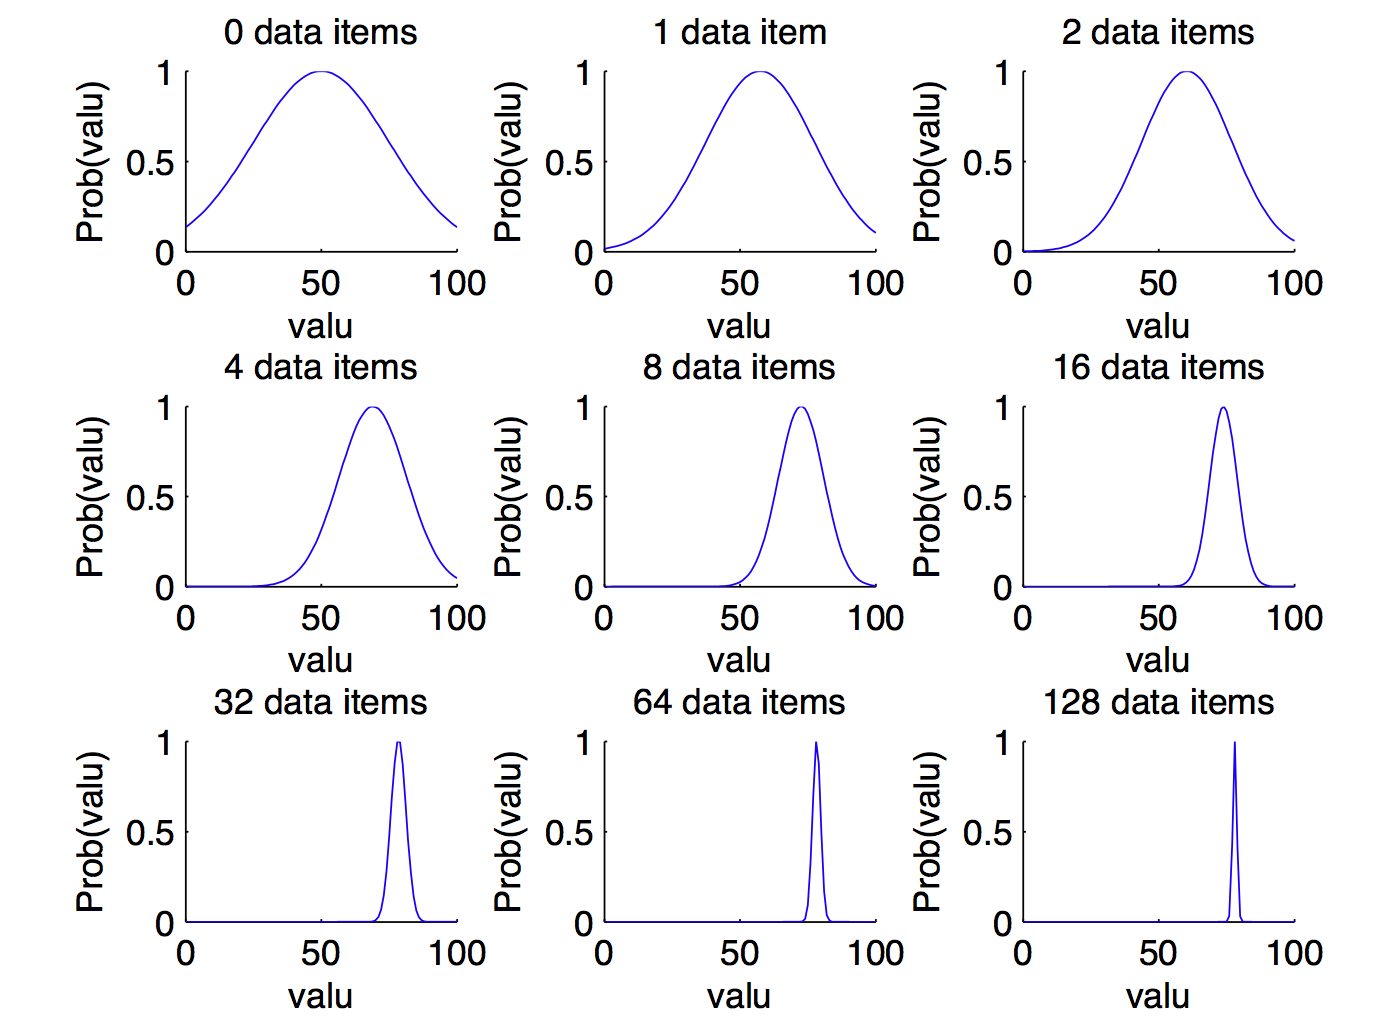
\includegraphics[width=0.7\textwidth]{graphics/sampling.png}
\begin{tiny}
\caption{Sampling and updating posterior probability density function of a normal distribution $\mathcal{N}\left( \mu , \sigma^2 \right)$. Figure taken from~\citep{Jacobs2008normalnormal}.\label{fig:sampling}}
\end{tiny}
\vspace{1cm}
\end{figure}


\subsection{Introduction to Thompson Sampling\label{sec:thompson}}
Thompson Sampling was first proposed in 1933 by William R.\ Thompson~\citep{thompson:biom33} and mainly concerned Bernoulli processes. In this section we explain this approach and discuss related work extending originally proposed methodology~\citep{May:2012:OBS:2503308.2343711}. Furthermore, it can be proved that under presented below assumptions the approach behaves optimally.\\
Described here solution is widely used for on-line advertising by IT giants like Microsoft, Google and Yahoo due to its simplicity, flexibility and scalability~\citep{graepel2010web}. Moreover, simulations indicate superiority of Thompson Sampling over all competitors~\citep{May:simulation}.\\


% \subsubsection*{Introduction}
% Firstly the general idea is presented. 


\subsubsection{Intuition}
We will begin with intuitive description of mechanisms ruling the process.\\
With a view of clarifying we assume that at each time step we are able to obtain a sample from posterior distribution with mean $\mu_a$ and variance $\sigma_a$ for each action $a$. If our goal is to maximize the reward we simply select the arm with highest local reward(highest sample). If all assumptions about our process hold by selecting given action we improve our estimate of its parameters. It is desirable to incorporate obtained sample and update mean and variance---therefore our posterior becomes a prior for the next round.\\

In order to visualize this we assume that we have 2 arms; the posterior of first one is always less than of the second one and the later behaves as shown in figure~\ref{fig:sampling}. We can see that as we sample and update the posterior it converge to true mean and simultaneously the variance of our estimate decreases. It is clear that we can only update the estimate of selected action and no other.\\

Usually, drawn sample will be quite close to mean~\ref{fig:sim1}(normal distribution) yielding choice of action with highest mean; occasionally it will lie in the distribution tail leading to exploration of suboptimal at given time action~\ref{fig:sim2}. In other words, the higher the variance of action, the greater the probability of exploring particular arm. This argument intuitively guarantees infinite exploration of environment thus convergence to overall optimal solution.


\begin{figure}[htbp]
\centering
  \begin{subfigure}[b]{0.49\textwidth}
    \centering
    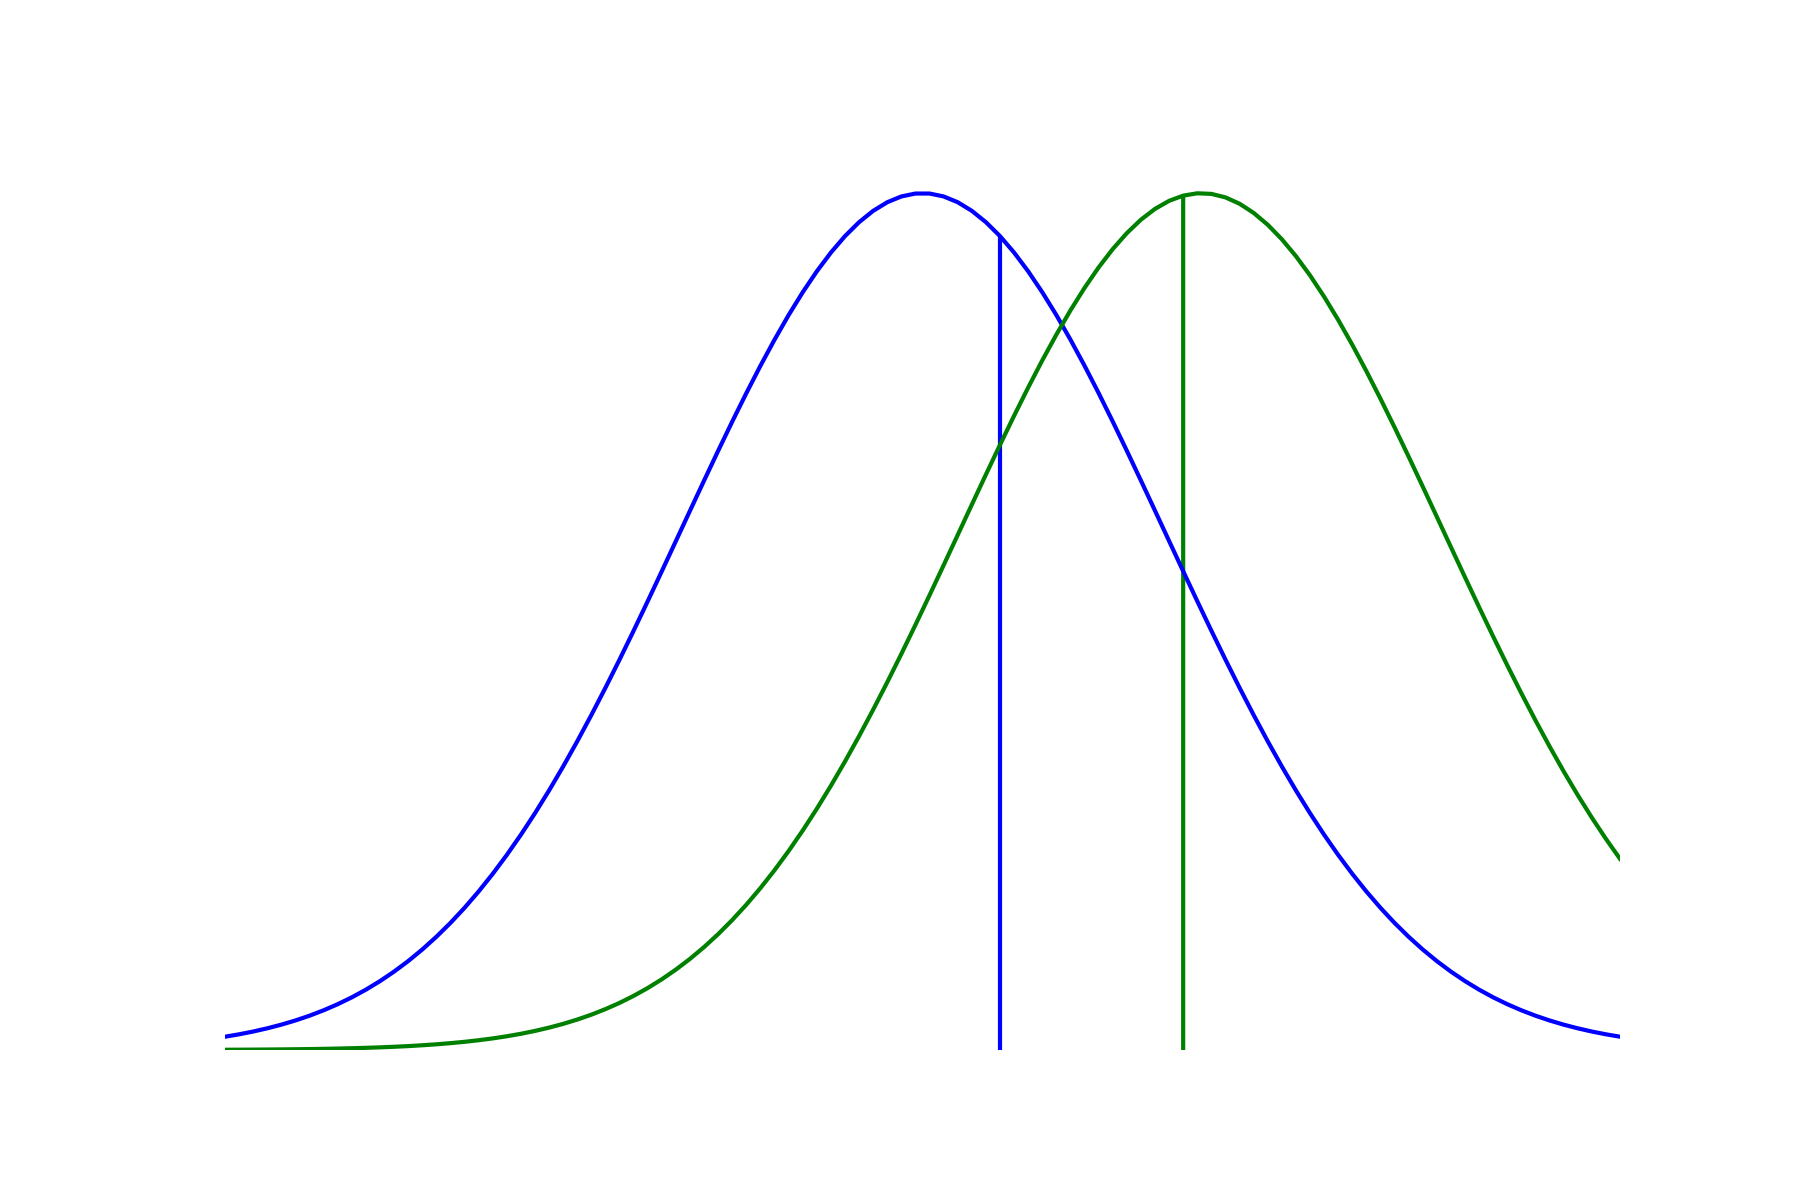
\includegraphics[width=0.99\linewidth]{graphics/sim1.png}
    \caption{\label{fig:sim1}}
  \end{subfigure}
  \begin{subfigure}[b]{0.49\textwidth}
    \centering
    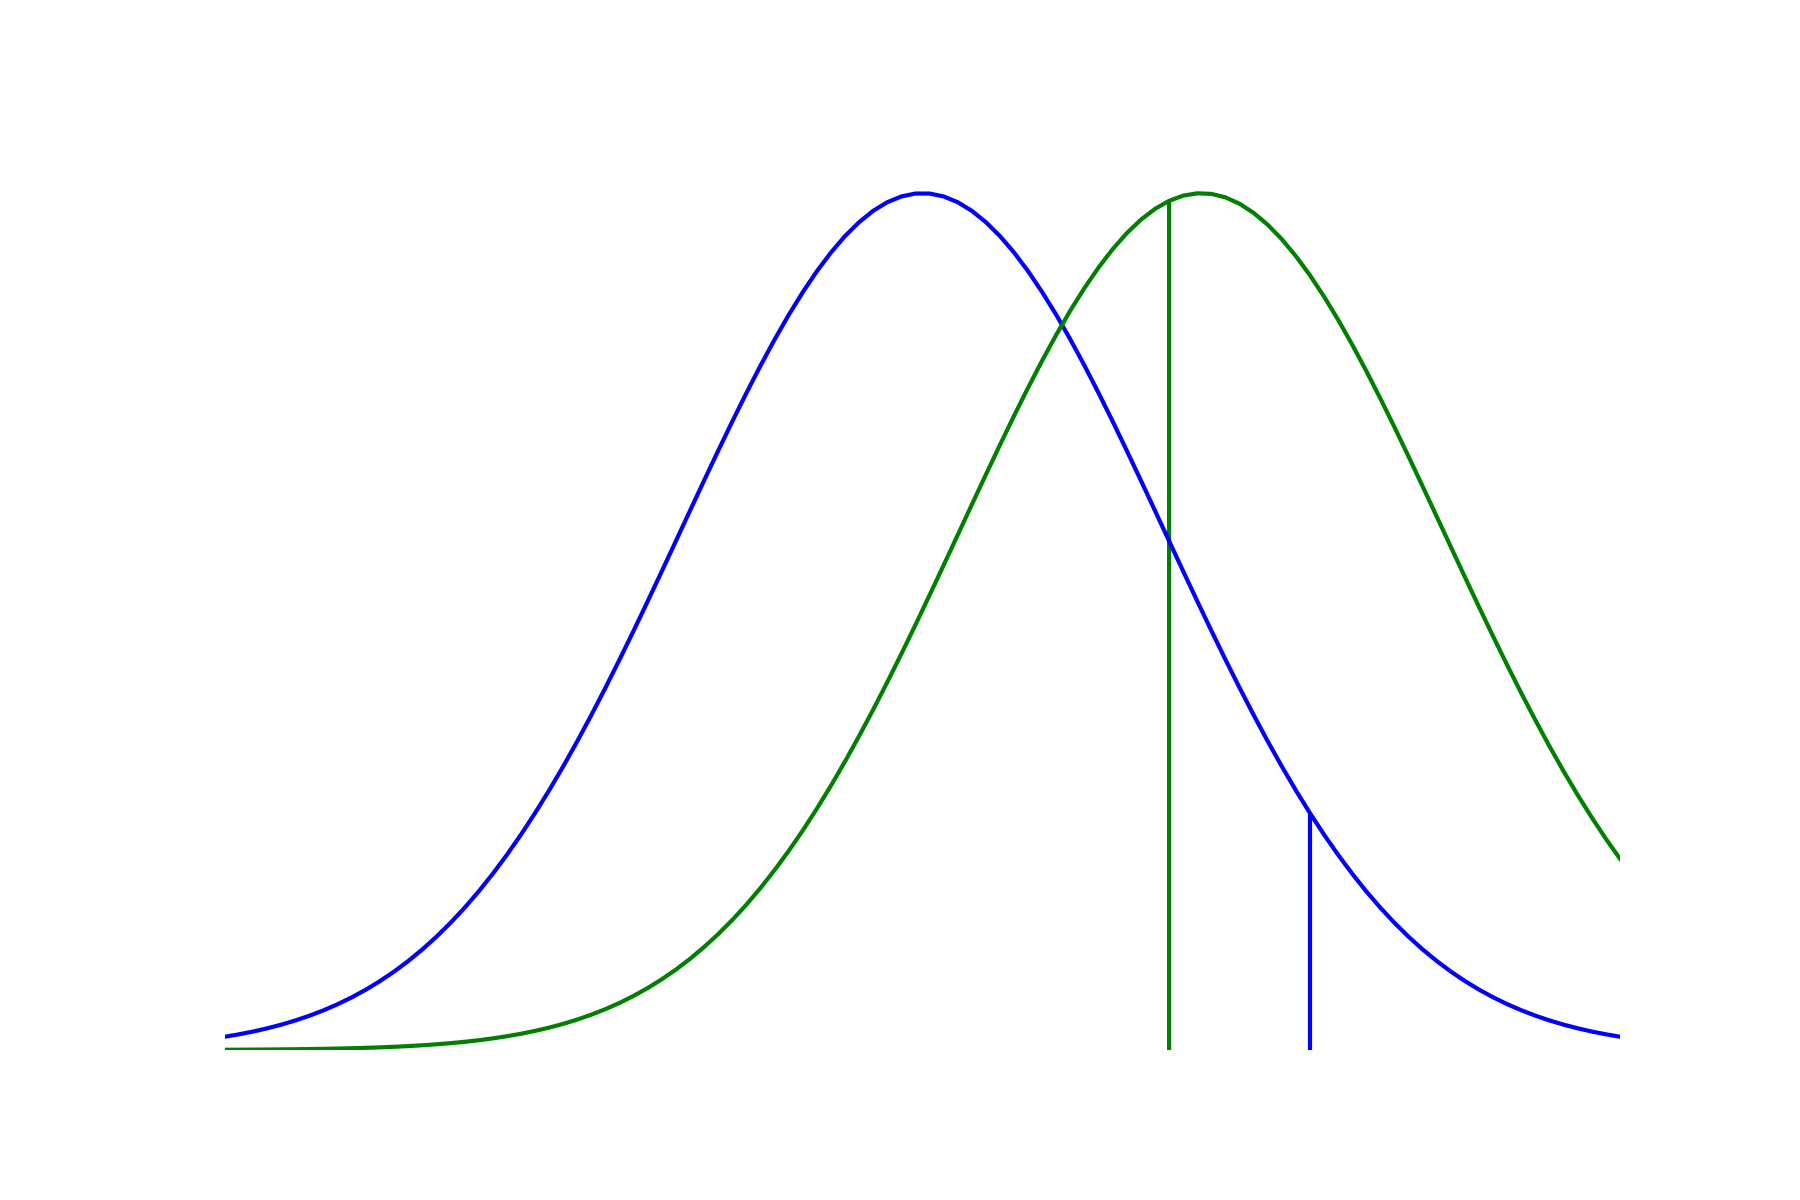
\includegraphics[width=0.99\linewidth]{graphics/sim2.png}
    \caption{\label{fig:sim2}}
  \end{subfigure}
\begin{tiny}
\caption{Sampling from two posteriors of normally distributed arm.\label{fig:sim}}
\end{tiny}
\vspace{1cm}
\end{figure}


\subsubsection{Example}
Lets assume we are given uniform prior and we model each arm as normally distributed with unknown mean $\mu_a$ and known variance $\sigma^2_a$. Ties are broken randomly; we choose any action in the first round.\\

We generate normal posterior according to theory presented in section~\ref{sec:bayesian}.\\

After we have obtained posterior we draw a sample for each arm $\mathit{s}_a \leftarrow \mathcal{N}(\mu_a^{\texttt{ pos}}, \sigma^{2\texttt{ pos}}_a)$.\\

Our selection procedure is $\mathit{a}_{t+1} = \operatorname{arg\,max}_{a \in \mathscr{A}} \mathit{s}_a$. So we play an arm $s$ in round $t+1$ and repeat previous steps. We place all outcomes and samples in the history vector.\\


\subsubsection{Assumptions}
In our considerations the process runs for an infinite sequence of \emph{time steps}, $t \in \mathscr{T} = \{ 1,2,3... \}$; at each step we observe \emph{regressor}, $x_t \in \mathscr{X}$ (compact set); an \emph{action} choice at time $t$ is $a_t \in \mathscr{A} = \{ 1,2...A \}$ and $A<\infty$.\\
Furthermore action selection is based on \emph{information sequence}(history vector) defined as:
$$
  \tilde{\mathscr{L}}_t = \left( \text{  } (x_1,a_1,r_1);...(x_{t-1},a_{t-1},r_{t-1}) \text{  } \right) \text{ ,}
$$
where $x$ and $a$ is defined as above, $r$ is a reward which results from action at given time and $r_t = f_{a_t}(x) + z_{t,a_t}$; the later value in the sum is i.i.d.\ \footnote{independent and identically distributed} random variable with unknown distribution, zero mean and finite variance. We also denote information available prior to experiment as $\mathscr{L}_0$ and information at time $t$ as $\mathscr{L}_t = \left( \mathscr{L}_0 \cup \tilde{\mathscr{L}}_t \right)$.\\
Finally, $f_a : \mathscr{X} \rightarrow \mathbb{R}$ is an unknown continuous function of the regressor specific to the action $a$.\\



We can therefore define the optimal action---with highest expected reward---at time $t$ by:
\begin{equation}
  a_t^\star = \argmax_{a \in A} f_a (x_t) \text{ ,}
\end{equation}
and its approximation by:
\begin{equation}
  \label{eqn:optsol} \hat{a}_t^\star = \argmax_{a \in A} \hat{f}_a (x_t) \text{ .}
\end{equation}

We can prove that this policy converges with time to the best possible policy(infinite selection of arm with highest reward)---\emph{convergence criterion}:
\begin{equation}
  \label{eqn:convg}
  \frac
    {\sum_{s=1}^t f_{a_s} (x_s)}
    {\sum_{s=1}^t f^\star (x_s)}
  \xrightarrow{\text{ a.s.\ }} 1 \text{ as } t \rightarrow \infty \text{ .}
\end{equation}
Above formula states that in infinite process we will finally discover the optimal arm and we will be playing it forever since.\\


We need to consider two major steps of constructing such policy: action evaluation and selection schemes. We also require that evaluation function is \emph{consistent}.\\

To achieve consistency we need to guarantee:
$$
  \forall a \in A \text{, } \forall x \in X \text{, } \left[ \hat{f}_{t, a}(x) - f_a(x) \right] \xrightarrow{\mathbb{P}} 0 \text{ as } n_{t,a} \rightarrow \infty \text{ .}
$$
Here consistency means that by improving our estimate of regressor function after each selection and information gain we will finally get really close to the true function.\\

Even though we guarantee consistent estimator it is possible that optimal action will never be selected. This feature of solution requires as to make sure that arms seen as sum-optimal will also be explored. The solution is to ensure infinite exploration:
$$
  \mathbb{P} \left( \bigcap_{a \in A} \left\{ n_{t,a} \rightarrow \infty \text{ as } t \rightarrow \infty \right\} \right) = 1 \text{ .}
$$
The above equation tells us that the number of times each action is selected tends to infinity as the process continues in time.\\ 

Finally, we want the action(arm) selection process to exploit obtained information. We want it to be greedy \footnote{Locally optimal choice at each stage.} in the limit. This assumption leads to:
$$
  \mathbb{P} \left( a_t = \hat{a}_t^\star | \mathscr{L}_t, x_t \right) \xrightarrow{\text{a.s.\ }} 1 \text{ as } t \rightarrow \infty \text{ ,}
$$
where $\hat{a}_t^\star$ is defined as in equation~\ref{eqn:optsol}. The above equation means that the action that our policy estimate as optimal will be truly optimal in the time limit.\\

If all above conditions hold we call the policy \emph{GLIE}---greedy in the limit with infinite exploration.\\


\subsubsection{Exploration and exploitation}
Action selection mechanism uses sum of \emph{exploitative} and \emph{exploratory} values to make a greedy decision at each time step. The first quantity corresponds to immediate reward---expected value of posterior distribution for each action at given time---and we define it as:
\begin{equation}
  \label{eqn:exploitative} \hat{f}_{t,a} (x_t) = \mathbb{E} ( f_a(x_t) | \mathscr{L}_t, x_t ) \text{ .}
\end{equation}
The exploratory parameter can be expressed in many different ways reviewed by~\citep{meuleau:exploration}. Broadly speaking, this value describes how keen we should be on exploring other than optimal actions; it can be defined as:
$$
  \delta_{t,a} \myeq
    \begin{cases}
     \sigma_{t,a} \delta_0(\mathscr{L}_t) & \text{for known variance,}\\
     s_{t,a}      \delta_0(\mathscr{L}_t) & \text{for unknown variance,}
    \end{cases}
$$
where $\delta_0(n)$ is some positive decreasing function of \emph{history} called \emph{unit exploration bonus}.\\

$\delta_0$ for instance can be dependent on discount sequence: decreasing the importance of exploration later in the experiment or giving the same priority to exploration independently of time. Moreover, the \emph{exploratory bonus} can be calculated simply as standard deviation of the expected reward(of posterior distribution of each action). Such approach favours actions which predictions are uncertain hence, improve their true reward estimation.\\

\subsubsection{Approach development}
We now refine described above approach and present \emph{Local Thompson Sampling}(LTS). To begin with, we design exploratory value in a way that will guarantee non-sticking~\footnote{Avoid focusing on one action hence under-explore all the other(sub-optimal solution).}. One solution is to randomize it. Such behavior can be achieved by sampling from the posterior distribution and using acquired quantities as an error in exploitative value estimate for current regressor; we denote $\tilde{f}_{t,a}^{\text{ Th}} (x_t)$ as sample from posterior distribution of $f_a(x_t) - \hat{f}_{t,a}(x_t)$, given $\mathscr{L}_t$ and $x_t$:
\begin{equation}
  \label{eqn:exploratory} \tilde{f}_{t,a}^{\text{ Th}} (x_t) \sim \{ f_a(x_t) - \hat{f}_{t,a}(x_t) \} | \mathscr{L}_t,x_t \text{ .}
\end{equation}
Intuitively, $\hat{f}_{t,a}(x_t)$ is our estimate of the mean of true function based on all the information and regressors that we observed so far; $f_a(x_t)$ is the true function of the regressor. The sampled value from the distribution given by difference of these two functions provides us with estimate of uncertainty of given action which is random.\\

Sum of both exploratory and exploitative values given in equations~\ref{eqn:exploratory}~and~\ref{eqn:exploitative} is used in LTS to greedily decide on the next action; this process is equivalent to choosing an action with optimal posterior probability for current regressor. It can be expressed as sampling from:
$$
\{ f_a(x_t) - \hat{f}_{t,a}(x_t) \} +  \mathbb{E} ( f_a(x_t) | \mathscr{L}_t, x_t )
=
 \{ f_a(x_t) - \hat{f}_{t,a}(x_t) \}+ \hat{f}_{t,a} (x_t)
 =
 f_a(x_t) \text{ ,}
$$
which is just a posterior distribution of an action $a$.\\
As we do not have the true function $f$ for arm $a$ the closest approximation is posterior distribution. Therefore, the policy says to sample from the posterior distribution and choose the arm with highest sample.\\
It is proved that in LTS algorithm probability of each action being selected is the posterior that the action is yielding the highest expected reward. Furthermore, we assume that posterior of all actions that have not been taken at round $t$ does not change.\\

We call this approach \emph{local} as it uses greedy action selection---the choice is made based on probabilities calculated for current regressor. The original work by Thompson discussed only Bernoulli bandits but as shown above it can be generalized to sample from the posterior distribution of the expected reward of each action and then select the arm with highest value.\\

Under mild assumptions~\footnote{Assumptions that are expected to hold if the true posterior distributions and expectations are available.} it can be shown that LTS guarantees convergence given by equation~\ref{eqn:convg}. Such solution was first proposed by Thompson~\citep{thompson:biom33}.\\

% \subsubsection{Correctness \& convergence} %LTS and OBS are myopic methods.
% Sampling from sum of exploratory and exploitative values given in equations~\ref{eqn:exploratory}~and~\ref{eqn:exploitative} yield:
% $$
  % \left[ f_a(x_t) - \hat{f}_{t,a}(x_t) \right] + \hat{f}_{t,a}(x_t) = f_a(x_t) \text{ .}
% $$

\RestyleAlgo{boxed}
\vspace{2cm}
\begin{algorithm}[H]
  \KwData{Posterior distributions for each action---$\left\{ p_a(\cdot|\mathscr{L}_t,x_t) : a \in \mathscr{A} \right\}$}
  \For{$a \in \mathscr{A}$}{
    \text{sample: }$\mathscr{Q}^\text{Th}_{t,a} \leftarrow p_a(\cdot|\mathscr{L}_t,x_t)$ \;
  }
  sample $a_t$ uniformly from $\operatorname{arg\,max}_{a \in \mathscr{A}} \mathscr{Q}^\text{Th}_{t,a}$ \;
 \caption{Local Thompson Sampling(LTS).\label{al:LTS}}
\end{algorithm}
\vspace{2cm}

We denote $p_a(\cdot | \mathscr{L}_t, x_t)$ the posterior distribution of $f_a(x_t)$ given $\mathscr{L}_t$ and $x_t$ and $\mathscr{Q}^\text{Th}_{t,a}$ a random variable with distribution $p_a(\cdot | \mathscr{L}_t, x_t)$ which we draw our samples from.\\


\subsubsection{Drawbacks and possible improvements}
Main disadvantage of this approach is possibility of exploratory value having zero expectation hence, it can be negative. The consequence may lead to probability of particular action being selected to decrease with the posterior variance of its exploratory value.\\
This issue arises as we represent the samples as sum of exploratory and exploitative values therefore if actions with the highest exploitative value has a lot of uncertainty then it is less likely to be played then if the estimate had little uncertainty.\\

The approach which avoids such situations is called \emph{Optimistic Bayesian Sampling}(OBS) where exploratory value is given by:
$$
  \tilde{f}_{t,a} (x_t) = max \left( 0, \tilde{f}_{t,a}^{\text{ Th}} (x_t) - \hat{f}_{t,a}(x_t) \right)
                        = \left [ \tilde{f}_{t,a}^{\text{ Th}} (x_t) - \hat{f}_{t,a}(x_t) \right]_+
                        \text{ .}
$$
Expressed in this way exploratory value has positive expectation and cannot be negative. This feature yields increased selection of uncertain actions---what seems desirable. It also can be shown that OBS satisfies convergence criterion(equation~\ref{eqn:convg}) and outperforms LTS~\citep{May:2012:OBS:2503308.2343711}.\\

\RestyleAlgo{boxed}
\vspace{2cm}
\begin{algorithm}[H]
  \KwData{Posterior distributions for each action---$\left\{ p_a(\cdot|\mathscr{L}_t,x_t) : a \in \mathscr{A} \right\}$}
  \For{$a \in \mathscr{A}$}{
    \text{sample: }$\mathscr{Q}^\text{Th}_{t,a} \leftarrow p_a(\cdot|\mathscr{L}_t,x_t)$ \;
    $\hat{f}_{t,a} (x_t) \leftarrow \mathbb{E}( \mathscr{Q}^\text{Th}_{t,a} | \mathscr{L}_t,x_t )$ \;
    $\mathscr{Q}_{t,a} \leftarrow \operatorname{max}(\mathscr{Q}^\text{Th}_{t,a}, \hat{f}_{t,a} (x_t))$ \;
  }
  sample $a_t$ uniformly from $\operatorname{arg\,max}_{a \in \mathscr{A}} \mathscr{Q}_{t,a}$ \;
 \caption{Optimistic Bayesian Sampling(OBS).\label{al:OBS}}
\end{algorithm}
\vspace{2cm}

\subsubsection{Conclusions}
Presented here class of algorithms is robust---as long as relevant assumptions hold, convergence criterion is satisfied even if approximations of posteriors and expectations are used. Above algorithms are also easy to implement given that posterior distribution of expected rewards can be calculated. Furthermore, the method is computationally cheap in comparison with belief-lookahead approaches such as Gittins index. Last but not least, LTS is widely used by Microsoft, Google and Yahoo to address contextual bandit problem.\\




\chapter{\texttt{\textbf{Exploitation}}---Practical application\label{ch:MAB-AL}}

There is a number of historical applications of multi-armed bandits (MAB) mainly concerned with research time management, general job-scheduling, economics and military~\citep{gittins+glazebrook+weber}.
Nowadays, one of main utilisations is found in contextual bandits which are foundation for optimizing online advertising income. The general idea behind this concept is to present different variations of ads layout at given webpage which are suited to user by inspecting one's history and are widely used by IT giants like Google, Yahoo, Facebook, LinkedIn or Microsoft. For majority of these companies the theory is of high interest as lion's share of their revenue flows from click-through rate in online advertising.~\citep{graepel2010web, Scott:2010:MBL:1944422.1944432}\\

Another application presented in~\citep{Antos09activelearning} describes how to apply well known in machine learning approach: \emph{active learning} to estimate mean of finite number of arms to achieve equally good estimation of these values. Authors claim described problem is of high interest while considering quality control with multiple production lines; proposed solution gives guideline how often company should check products from particular machine.\\
In this chapter we will look at this problem the other way around, namely: how can we generalise multi-armed bandit framework to create efficient and robust active learning algorithm.\\

Other, most recent application of MAB theory in computer science is concerned with classification issue in environment of insufficient information. This approach to machine learning field seems to be under-explored and needs more attention from a research world as to the best of our knowledge it was addressed so far in only one scientific publication, namely~\citep{DBLP:journals/corr/GantiG13}.\\
Our decision was to pursue this topic mainly by presenting here deep analysis of chosen in~\citep{DBLP:journals/corr/GantiG13} approach. After broad explanation we seek for potential improvements and alternatives of presented algorithm.

\section{Structure of this chapter}
We first introduce foundations of machine learning needed to develop concepts of semi-supervised (SSL) and active (AL) learning. Next, we introduce whole family of active learning scenarios and give detailed description of the one needed for understanding~\citep{DBLP:journals/corr/GantiG13}. Then, we present possible connection between processes of MAB and AL. This interface, will allow to frame active learning as a bandit process.\\
Proceeding, main section of this chapter focuses on described in \citep{DBLP:journals/corr/GantiG13} ``bridge'' connecting both worlds. Finally, we explore potential changes that can be introduced and improvements that can be beneficial for described earlier algorithm.
%explore in great detail

\section{Machine Learning 101}
\subsection{General Learning}
Machine Learning is a field of Computer Science which is mainly concerned with building a model for a given data. Classification problem is of the form $\mathit{l} : \mathscr{X} \rightarrow \mathscr{Y}$, where $\mathscr{X}$ is called \emph{instance space} and $\mathscr{Y}$ is \emph{output space} --- in supervised scenario often replaced with $\mathscr{L}$ and called \emph{label space}.\\
Such function $\mathit{l}$ is called \emph{model}, which we try to approximate. The instances which are supplied to the model are preprocessed to extract \emph{features}, which represent each instance in a form of a vector describing chosen attributes. Based on feature vector given model assigns the element to particular region in output space; or in case where $\mathscr{Y} = \mathscr{L}$ gives the instance chosen label.\\

In classical scenario called \emph{supervised learning} the approximation of model(~$\mathit{\hat{l}}$~) is generated by supplying pairs $(\mathit{\mathbf{x}}, \mathit{y})$ which belong to dataset called \emph{training set} where $\mathit{\mathbf{x}}$ is feature vector and $\mathit{y}$ is target label.\\
In general supervised learning is one of the most common scenarios and is concerned with finding a \emph{class} for a given exemplar. Widely used in literature example is to build a model which predicts whether a particular e-mail is spam or non-spam based on extracted features i.e.\ words from the content of the message.\\

Another important building block of machine learning theory is the concept of evaluating accuracy or performance of a trained model. The most popular measure in presented above supervised scenario is so called error rate. It is calculated using \emph{test set} which is disjoint with training set i.e.\ unseen by trained model. Typically the value is calculated as $\mathtt{Err} = \frac{\text{incorrectly classified instances}}{\text{all instances}}$.\\

In different words, the main goal of machine learning is to choose some \emph{hypothesis} from \emph{hypothesis space} which best ``fits'' given data sample. For our purposes we generalise hypothesis space to a set of all possible assignments of classes to training data points.\\
For instance if we are given (in fixed order) three data points $(x_1, x_2, x_3)$ and our task is binary classification i.e.\ we either predict $+$ or $-$, our hypothesis space is then $H = {(+, +, +), (+, +, -), (+, -, +), (-, +, +), (+, -, -), (-, +, -), (-, -, +), (-, -, -)}$.\\

If we discuss performance of given hypothesis more sophisticated measure of uncertainty is \emph{loss function} $L : \mathbb{R} \rightarrow [0, \infty)$ which maps \emph{margin} $z(\mathbf{x})$ of particular exemplar to an associated loss $L(z(\mathbf{x}))$. It is primarily used in scoring and ranking classifiers.\\
By utilising ranking value and true class information we construct a margin which can be understood as the higher positive value the better the model fits for the exemplar; the lower negative value the worse the model fits for the exemplar.\\
The loss function rewards large positive margins and penalises large negative values. Often we assume $L(0) = 1$ what gives a loss of an exemplar on decision boundary, $L(z) \geq 1$ for $z < 0$ and $0 \leq L(z) < 1$ for $z > 0$. Sometimes the quantity of interest is average loss over test set \texttt{Te} calculate as $\mathtt{Te} = \frac{1}{|\mathtt{Te}|} \sum_{x \in \mathtt{Te}} L(z(\mathbf{x}))$.\\
The simplest loss function called \emph{0--1 loss} is defined as:
\[
 L_{\text{0--1}} (z) =
  \begin{cases}
   1 & \text{for } z \leq 0 \\
   0 & \text{for } z > 0 \text{.}
  \end{cases}
\]~\\
We have already seen average 0--1 loss as an error rate \texttt{Err}:
\[ \frac{1}{|\mathtt{Te}|} \sum_{x \in \mathtt{Te}} L_{\text{0--1}}(z(\mathbf{x})) = 
   \frac{1}{|\mathtt{Te}|} \sum_{x \in \mathtt{Te}} \mathds{1} \left[ z(\mathbf{x}) \leq 0 \right] =
   \frac{1}{|\mathtt{Te}|} \sum_{x \in \mathtt{Te}} \mathds{1} \left[ \text{incorrectly classified instance?} \right] =
   \mathtt{Err}\text{.}
\]~\\

Some other popular loss functions are:
\begin{description}
\item[hinge loss] $L_{\text{h}} (z) = 1 - z$ for $z \leq 1$ and $L_{\text{h}} (z) = 0$ for $z > 1$,
\item[logistic loss] $L_{\text{log}} (z) = \log_2 (1 + \exp(-z))$,
\item[exponential loss] $L_{\text{exp}} (z) = \exp(-z)$,
\item[squared loss] $L_{\text{sq}} (z) = (1 - z)^2$; which sometimes is equated to $0$ for $z>1$.\\
\end{description}

One way of categorizing classification in predictive scenarios is based on task:
\begin{description}
\item[Classification] finding a label to describe instance(e.g.\ spam / non-spam),
\item[Scoring and ranking] for each instance outputs score vector over all classes,
\item[Probability estimation] for each instance outputs probability vector over all classes,
\item[Regression] learn approximation to the true labeling function.\\
\end{description}

As mentioned earlier there are a few scenarios used in ML. Main settings of machine learning can be divided by two criteria. Namely the form of supplied training data: whether it is labeled --- \emph{supervised} learning or unlabeled --- \emph{unsupervised} learning and the goal of classification: whether process aims at predicting a target variable(most often label) --- \emph{predictive} model or discover the structure of the data(describe the underlying format) --- \emph{descriptive} model.\\

\begin{table}[htbp]
  \begin{tabular}{ r | c p{5cm} }
                         & Predictive models          & Descriptive models \\
    \hline
    Supervised learning   & classification, regression & subgroup discovery \\
    Unsupervised learning & predictive clustering      & descriptive clustering, association rule discovery \\
  \end{tabular}~\\[0.1cm]
  \caption{Main learning models in ML.\label{fig:learning_models}}
\end{table}~\\

The main reference for further reading is~\citep{flach2012machine} containing comprehensive introduction to machine learning.


\subsection{Semi-supervised Learning}
There is a missing link in the chain which, connects supervised and unsupervised scenarios called \emph{semi-supervised} learning (Table~\ref{fig:learning_models}). The goal of such classification is to train classifier on relatively small sample of labeled data in a way that its performance on unseen data is close to one that we could achieve with supervised algorithm using huge sample of labeled data. The general strategy is to use the most informative points which best describe distribution underlying classes in the data.\\
The issue with such approach is difficulty of acquiring such points. Provided data can be noisy --- contain outliers due to measurement errors therefore we need to have enough of them to estimate these values from sample.\\
There are many algorithms which build models based on small sample of labeled data but minority of them measure and utilize information about exemplars being maximally informative to improve model they output.\\

The main application area of semi-supervised learning is natural language, video or audio processing same as other fields where data are relatively easy to acquire --- for instance by placing camera in a public place, hours of material can be recorded --- but the process of labeling gathered data to find good fitting supervised model is expensive, time consuming or demand hours of manual labour.\\
The hidden concept is to describe small fraction of data by hand to train semi-supervised model which performs similarly to supervised algorithm in terms of error rate on data.

\subsection{Active Learning}
AL approach is considered as a special case of Semi-supervised learning. What differentiates these two models is the way initial training sample is organised. In S-SL algorithm is supplied with labeled data and does not have influence on what these data is and how it was chosen from the whole pool. On contrary, in AL the learner can choose whether it wants to know label of particular instance that it has access to. If algorithm is interested in label of chosen exemplar it queries so called \emph{label oracle} denoted by $\mathscr{O}$ to acquire it. We assume that if one point is queried more than once $\mathscr{O}$ will return always the answer it gave for the first query. Most often to produce a good oracle output the average label assigned by some expert population is chosen.\\

The major advantage of such approach is selectiveness of label information. The learner is not fed with fixed data where there is no possibilities to investigate potentially interesting hypothesis which are lacking evidence to be supported. It has free will which is most often managed via some kind of hypothesis risk minimisation techniques.\\

Within active learning we can name different scenarios of querying $\mathscr{O}$. We can distinguish algorithms based on:
\begin{description}
\item[Membership Query] the learner can query $\mathscr{O}$ for any point in input space $\mathscr{X}$ where $x$ does not necessarily belong to support of marginal distribution i.e.\ it is not in our training set,
\item[Stream Query] the learner sample points from marginal distribution one after another and decide on-the-fly whether to acquire its label or not,
\item[Pool Query] the learner has access to unlabeled \emph{pool} $\mathscr{P} = \left\{ \mathbf{x}_1, \mathbf{x}_2, \dots \mathbf{x}_{n-1}, \mathbf{x}_n \right\}$ of exemplars sampled from some marginal distribution. The learner is allowed to query $\mathscr{O}$ for a label of chosen point i.e.\ acquire $y \sim P_{Y|\mathscr{X} = \mathbf{x}}$.\\
\end{description}

We also need to make a decision about the strategy of finding best hypothesis. There are two main approaches: exploiting (cluster) structure in data and efficient search through hypothesis space. The first one boils down to clustering exemplars based on some distance measure between them and sampling number of points from each cluster to arrive at label (see Figure~\ref{fig:cluster}). The later one is organised in systematic manner search algorithm that outputs hypothesis fitted to given data (see Figure~\ref{fig:hypsearch}).\\

From this point onward we are narrowing our focus to \textbf{hypothesis space searched, active learning algorithms based on pool queries}.\\

\begin{figure}[htbp]
\centering
  \begin{subfigure}[b]{0.3\textwidth}
    \centering
    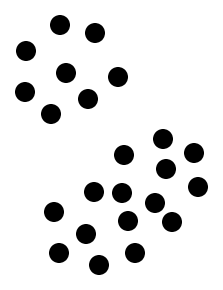
\includegraphics[width=0.5\linewidth]{graphics/cluster1.png}
    \caption{\label{fig:cluster_a}}
  \end{subfigure}
  \begin{subfigure}[b]{0.3\textwidth}
    \centering
    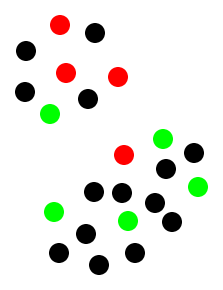
\includegraphics[width=0.5\linewidth]{graphics/cluster2.png}
    \caption{\label{fig:cluster_b}}
  \end{subfigure}
  \begin{subfigure}[b]{0.3\textwidth}
    \centering
    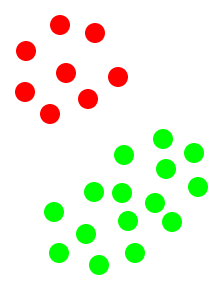
\includegraphics[width=0.5\linewidth]{graphics/cluster3.png}
    \caption{\label{fig:cluster_c}}
  \end{subfigure}
% 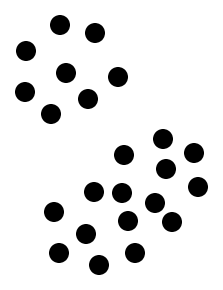
\includegraphics[width=0.3\textwidth]{graphics/cluster1.png}
% 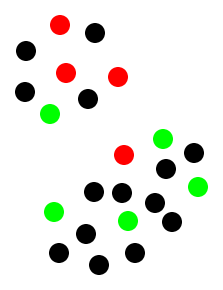
\includegraphics[width=0.3\textwidth]{graphics/cluster2.png}
% 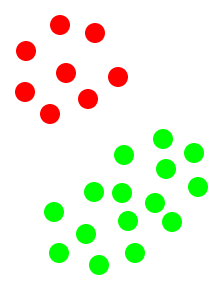
\includegraphics[width=0.3\textwidth]{graphics/cluster3.png}
\begin{tiny}
\caption{The process of exploiting cluster structure in data within active learning algorithm. In \ref{fig:cluster_a} we are supplied with some unlabeled data with obvious structure --- 2 clusters. In \ref{fig:cluster_b} we query for labels of some points from each cluster --- clusters are not pure, collected sample is noisy. In \ref{fig:cluster_c} we assign majority class to each cluster and arrive at presented model.\label{fig:cluster}}
\end{tiny}
\vspace{1cm}
\end{figure}


\begin{figure}[htbp]
\centering
  \begin{subfigure}[b]{0.3\textwidth}
    \centering
    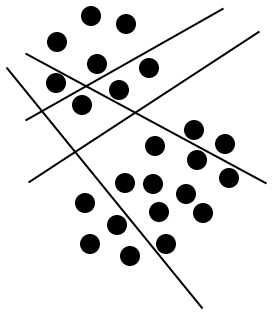
\includegraphics[width=0.5\linewidth]{graphics/hypsearch1.png}
    \caption{\label{fig:hypsearch_a}}
  \end{subfigure}
  \begin{subfigure}[b]{0.3\textwidth}
    \centering
    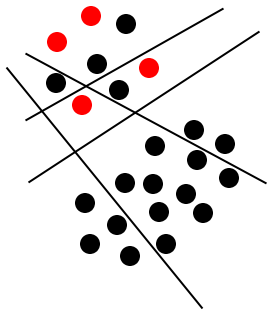
\includegraphics[width=0.5\linewidth]{graphics/hypsearch2.png}
    \caption{\label{fig:hypsearch_b}}
  \end{subfigure}
  \begin{subfigure}[b]{0.3\textwidth}
    \centering
    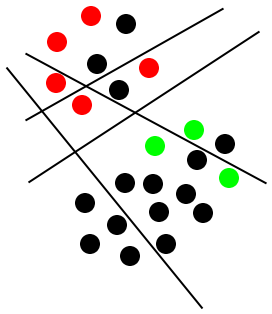
\includegraphics[width=0.5\linewidth]{graphics/hypsearch3.png}
    \caption{\label{fig:hypsearch_c}}
  \end{subfigure}
  \begin{subfigure}[b]{0.3\textwidth}
    \centering
    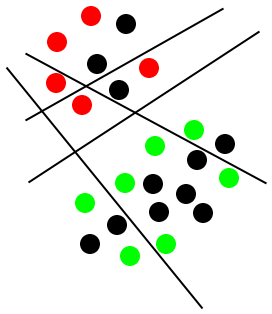
\includegraphics[width=0.5\linewidth]{graphics/hypsearch4.png}
    \caption{\label{fig:hypsearch_d}}
  \end{subfigure}
  \begin{subfigure}[b]{0.3\textwidth}
    \centering
    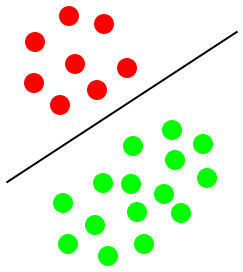
\includegraphics[width=0.5\linewidth]{graphics/hypsearch5.png}
    \caption{\label{fig:hypsearch_e}}
  \end{subfigure}
% 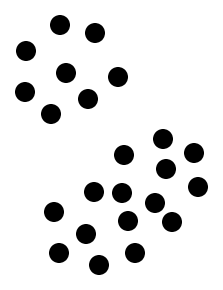
\includegraphics[width=0.3\textwidth]{graphics/cluster1.png}
% 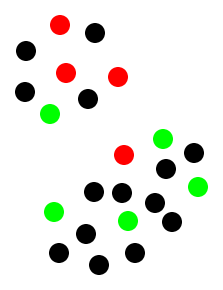
\includegraphics[width=0.3\textwidth]{graphics/cluster2.png}
% 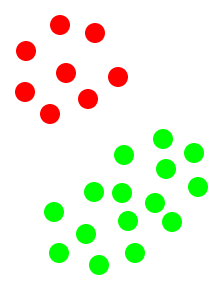
\includegraphics[width=0.3\textwidth]{graphics/cluster3.png}
\begin{tiny}
\caption{The process of search through hypothesis space within active learning algorithm. In \ref{fig:hypsearch_a} we select some hypothesis (~$h_i$~) that are potentially the best. To eliminate first we ask for a labels of points on both sides of $h_1$ and disregard it as on both sides we spot the same class (Figure \ref{fig:hypsearch_b}). In \ref{fig:hypsearch_c} and \ref{fig:hypsearch_d} we do the same for $h_2$ and $h_3$. We reject both of them with similar to previous observation. Finally, we arrive at hypothesis $h_5$ which agrees on all queried points and become output of our learning algorithm --- we assign to the rest of points majority class on given side of $h_5$.\label{fig:hypsearch}}
\end{tiny}
\vspace{1cm}
\end{figure}



\section{Active Learning in a view of Multi-Armed Bandits}
To build a ``bridge'' between MAB and AL we first need to describe settings of such scenario. For the sake of simplicity we focus on pool based, binary active learning with an approach of search through \emph{hypothesis space} $\mathscr{H}$, restricted by a query budget $B$. Moreover, we restrict our hypothesis space to linear classifiers(see later Section~\ref{sec:linearclassifiers}). The key point is to view learning problem as exploration-exploitation trade-off. We will first focus on finding connections between characteristic features of MAB and discover correspondence in AL.\\

To begin with, we will frame learning problem as $B$ round game --- finite horizon with discount sequence $\mathbf{A} = ( \underbrace{ 1, 1, 1, ..., 1}_{B}, 0, 0, 0, ... )$ --- where in each round agent is faced with pulling one of given arms and suffer some loss $L_t$ on chosen action. For simplicity, in this scenario we change reward for a loss what leads to optimal strategy being the one that minimizes loss instead of maximizing reward over $B$ rounds.\\

It is worth noting that if $B \rightarrow \infty$ then this becomes supervised algorithm which is fed by data stream.\\

To be more precise, we define equivalence between arms of a bandit and hypothesis $\mathit{h} \in \mathscr{H}$. We also need to find a proxy of MAB loss signal in our active learning scenario, but lets first clarify goals of our strategy.\\
The main aim is to estimate optimal hypothesis i.e.\ the one with lowest risk (loss) with use of as little labeled points as possible. If we knew the best $\mathit{h}$, so the one with minimal cumulative loss then the optimal strategy would be to pull this arm in each round of our experiment. This leads to the goal of finding optimal strategy as quickly as possible. Now we are left with defining a strategy telling us which arm to pull in each round and dilemma how to transform feedback --- in our case ground truth (genuine label) --- of queried point $x$ from our pull into a loss signal.\\

\subsection{Linear classifier\label{sec:linearclassifiers}}
To begin with, we define linear classifier as:
$$
c(x) = \mathbf{w} \cdot \mathbf{x} - t \text{~,~}
$$
where for binary classification we have:
$$
c(x) \geq 0 \rightarrow \text{ $x$ is assigned to $+$}
$$
$$
c(x) < 0 \rightarrow \text{ $x$ is assigned to $-$.}
$$\\

Where $\mathbf{w}$ is weight vector and $\mathbf{x}$ is data point with $\mathbf{x} \in \mathbb{R}^n$.\\
In general, linear model (hypothesis class) is concerned with finding the weight vector $\mathbf{w}$ such that our classifier is of the form given above. We can transform above equation to express decision boundary $t = \mathbf{w} \cdot \mathbf{x}$. This result tells us that decision boundary is a plane in the space spanned by $x_i \in \mathbf{x}$ variables. Where vector $\mathbf{w}$ is perpendicular to boundary and points in direction of $+$ class.\\
The notation of classifier can be simplified by extending both vectors $\mathbf{x}$ and $\mathbf{w}$ with $x_0 = 1$ and $w_0 = -t$ leading to decision boundary $c(x) = \mathbf{w}^{\circ} \cdot \mathbf{x}^{\circ} = 0$. In this form for the expense of one extra dimension we get decision boundary passing through origin of our coordinate system.\\
For visual example please see figure~\ref{fig:binclas}.\\

\begin{figure}[htbp]
  \centering
  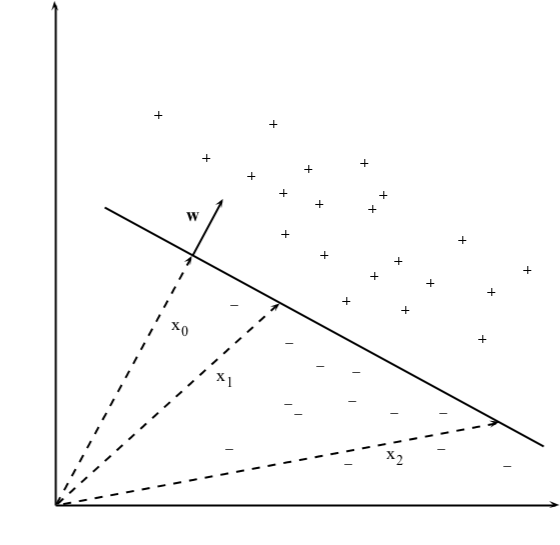
\includegraphics[width=0.5\linewidth]{graphics/binclas.png}
  \begin{tiny}
    \caption{Visualization of binary, linear classifier in two dimensions.\label{fig:binclas}}
  \end{tiny}
  \vspace{1cm}
\end{figure}

\subsection{Choosing best hypothesis\label{sec:risk}}
To address the first mentioned above issue we refer to~\citep{DBLP:journals/corr/GantiG13} where an unbiased estimator of the risk of hypothesis is defined as:\\
\begin{equation}\label{eq:mean}
\hat{L}_t(h) = \frac{1}{Nt} \sum_{n=1}^{N} \sum_{\tau = 1}^{t} \frac{Q^{\tau}_n}{p^{\tau}_n} L(y_n h(\mathbf{x}_n)) \text{~,}
\end{equation}
where $p^t_n$ is probability of querying $\mathbf{x}_n$ in round $t$ extracted from vector $p^t$ described in section~\ref{sec:pointtoquery}.\\
Furthermore, $Q^t_n$ is a random variable which takes values $\{0,1\}$; $1$ if $\mathbf{x}_n$ was queried in round $t$ and $0$ otherwise.\\

We also need to decide on loss function to employ in our model. All loss functions which are convex w.r.t\ margin and which are upper bounded by $L_{\text{max}} < \infty$ will be suitable. For example we could use logistic loss, squared loss or exponential loss.\\

To sum up, each hypothesis in group of linear classifiers can be fully describe by weight vector $\mathbf{w}$. This observation allows us to notationally unify output of hypothesis $h_j$ on point $\mathbf{x}_n$ as $h_j(\mathbf{x}_n) = \hat{c}(\mathbf{x}_n)$.\\


\subsection{Choosing a point to query --- Constructing loss signal\label{sec:pointtoquery}}
To iteratively improve our guess of best hypothesis we query possibly most informative point in each round. Intuitively such information allows us to tell apart good hypothesis which agree with acquired label and bad ones which mis-classify given point. To make the best possible choice we construct sampling distribution which minimizes the variance of the risk estimate $\hat{L}_t(h)$ defined above. We construct it by utilizing labels which we have already acquired from oracle and labels that our current hypothesis assigns to points which have not been queried yet. To guarantee infinite exploration of all hypothesis and avoid $0$ probabilities we introduce parameter $p_{min}$ which is arbitrarily set by user and denote minimum probability of each point being queried.\\

Let's define $\mathscr{Q}_t$ as a set of labels $y_n$ acquired by queering $\mathscr{O}$ for labels of $\mathbf{x}_n$ up to time $t$.\\
Just to recall we handle a binary classification which for data point $\mathbf{x}_n$ outputs result $c(\mathbf{x}_n)$. This result can be any real number, which is translated into class by rule given above: $c(\mathbf{x}_n) > 0 \rightarrow +$ and $c(\mathbf{x}_n) < 0 \rightarrow -$. As a notation shorthand it is often use $\textit{sign}(c(\mathbf{x}_n)) = y_n \in \{+, -\}$.\\

For each data point $\mathbf{x}_n \in \mathscr{P}$ in our pool we have:
$$
\hat{y}_n = \begin{cases}
                                    y_n = c(\mathbf{x}_n)  & \text{if } \mathbf{x}_n \in \mathscr{Q}_{t-1} \\
                                    \textit{sign}(h_t(\mathbf{x}_n)) & \text{otherwise.}
                                  \end{cases} 
$$

To decide which point to query we utilize introduced earlier loss and margin function; therefore setting $z(\mathbf{x}_n) = \hat{y}_n h_t(\mathbf{x}_n)$. Let's also note that cardinality of pool is: $|\mathscr{P}| = N$.\\
This leads to probability vector underlying sampling distribution being defined as:
$$
p_n^t = p_{\text{min}} + (1-Np_{\text{min}}) \frac{L(z(\mathbf{x}_n))}{\sum_{\mathbf{x}_n \in \mathscr{P}} L(z(\mathbf{x}_n))}
$$

Calculating $\hat{c}_t = h_t$ and $\\hat{y}$ for each $\mathbf{x}_n$ during arbitrary round $t$ allows us to utilize this information to calculate corresponding loss. The next stage is to create a vector $\mathbf{p}_t$ containing at n\ts{th} position $L(z(\mathbf{x}_n))$. Finally, we use it to construct sampling distribution to choose a point to query. Such approach has an advantage of being more prone to query points with small margin (large loss) w.r.t\ current hypothesis $h_t$ or points which have already been queried for label but on which $h_t$ suffers a large loss (simply does not agree).\\

After sampling $\mathbf{x}_n$ we check whether it was already queried in the past; if so we reuse already gained label. On contrary, if $\mathbf{x}_n$ has not been queried yet, we do so and increase our budget counter.


\subsection{Uncertainty of hypothesis\label{sec:uncertanity}}
The variance --- measure of uncertainty --- for risk (loss) of our hypothesis is calculated with help of calculated above vector for sampling distribution over pool instances as:
\begin{equation}\label{eq:variance}
U(\hat{L}_t(h)) = \frac{4}{Nt} \sqrt{\log\frac{1}{\delta}V_t}
\end{equation}
and
$$
V_t = \left[
\sum_{n = 1:N \\ \tau = 1:t} \frac{Q^\tau_n}{(p^\tau_n)^2} L^2(z(\mathbf{x}_n))
-
\left( \sum_{\mathscr{Q}_t} L(z(\mathbf{x}_n)) \right)^2
+
\frac{L^2_{\text{max}}  \sqrt{2t \log(\frac{1}{\delta}) (N-1)} } {\sqrt{p_{\text{min}}}}
\right]_+ \text{~,~}
$$

where $\delta$ is a parameter which is bounded by $\delta < \frac{1}{e}$.\\

This quantity together with previously defined estimator of the hypothesis risk was first defined in~\citep{DBLP:journals/corr/GantiG13}.\\


\subsection{Miscellaneous}
\subsubsection{Dealing with infinite hypothesis space}
Modeling huge or even infinite hypothesis space would suffer from existence of many arms in our bandit model leading to serious efficiency issue. Furthermore optimizing infinite space is not an easy task therefore we choose a subset of hypothesis space defined as:
$$
\mathscr{H} = \{ h : \|h\| \leq R \} \text{~,~}
$$
where $R$ is fixed such that $R > 0$ and $\| \cdot \|$ is Euclidean $L_2$ norm.\\
Furthermore, based on observation described in~\citep{Abernethy08competingin} we have self-concordant barrier $\mathscr{R}(h)$ on $\mathscr{H}$ defined as:
$$
\mathscr{R}(h) = - \log(R^2 - \|h\|^2) \text{~.~}
$$
Given above restrictions allow us to significantly reduce dimensionality of hypothesis space by choosing hypothesis which differ. Moreover, presented barrier function is a continuous function which penalize with value close to $\infty$ hypothesis approaching defined boundary of hypothesis space.\\


\section{MAB-AL Algorithm}

In this section we will briefly discuss \texttt{MAB-AL} algorithm proposed in~\citep{DBLP:journals/corr/GantiG13} to familiarize reader with general concept which build upon presented in previous sections milestones (see algorithm~\ref{al:LCB-AL}). \\Prior to classification the decision need to be made on loss function, query budget and lower bound on probability of each point being sent to oracle.\\

First of all, we initialize time and oracle queries counter variables and set our hypothesis to $0$ for each point --- classifier is maximally uncertain about label of each exemplar.\\

At the beginning of each round we construct label ($\{+, -\}$) for each point in our pool. If the point has already been queried we use its true label otherwise we assign label in agreement with current hypothesis. Then based on margin and loss we assign querying probability for each exemplar contributing to vector $\mathbf{p}^t$. We use $\mathbf{p}^t$ to create a sampling distribution and choose new point to query. For the sake of simplicity we allow exemplars to be re-queried so if the sampled point has already been sent to oracle we re-use previous label, otherwise we query oracle and increase our counter.\\

The heart of the algorithm is stated in line~\ref{al:LCB-AL:LCB} which performs \emph{Lower Confidence Bounds} calculation for all hypothesis in our $\mathscr{H}$. With freshly chosen $h$ we repeat above steps until we meet previously fixed budget, therefore picking hypothesis chosen during last iteration.\\

Details of summarized above approach are presented in~\citep{DBLP:journals/corr/GantiG13}.\\

\RestyleAlgo{boxed}
\vspace{2cm}
\begin{algorithm}[H]
 % \boxRuled
 \LinesNumbered
 \KwData{pool of points $\mathscr{P}$; loss function $L(\cdot)$; budget $B$; parameter $p_{min}$; access to oracle $\mathscr{O}$}
 \KwResult{optimal hypothesis $h_B$}
 $oracleQuerries = 0$\;
 $h_1 = 0$\;
 $t = 1$\;
 \While{oracleQuerries $\leq B$}{
  \For{$\mathbf{x}_n \in \mathscr{P}$}{
    $
    \hat{y}_n = \begin{cases}
      y_n = c(\mathbf{x}_n)  & \text{if } \mathbf{x}_n \in \mathscr{Q}_{t-1} \\
      \textit{sign}(h_t(\mathbf{x}_n)) & \text{otherwise.}
    \end{cases} 
    $ \;
    $p_n^t = p_{\text{min}} + (1-Np_{\text{min}}) \frac{L(z(\mathbf{x}_n))}{\sum_{\mathbf{x}_n \in \mathscr{P}} L(z(\mathbf{x}_n))}$ \;
  }
  sample point $\mathbf{x}$ from probability vector $\mathbf{p}^t$\;
  \eIf{$\mathbf{x} \in \mathscr{Q}_{t-1}$ --- was already queried}{
   reuse label of $\mathbf{x}$\;
   }{
   query oracle $\mathscr{O}$ for the label $y = c(\mathbf{x})$ of $\mathbf{x}$\;
   $\mathscr{Q}_{t} \leftarrow \mathscr{Q}_{t-1} \cup y$\;
   $oracleQuerries \leftarrow oracleQuerries + 1$\;
  }
  solve: $h_{t+1} \leftarrow \text{argmin}_{h \in \mathscr{H}} LCB_t(h) + \lambda_t \mathscr{R}(h)$\;\label{al:LCB-AL:LCB}
  $t \leftarrow t + 1$\;
 }
 \caption{LCB-AL presented in~\citep{DBLP:journals/corr/GantiG13}.\label{al:LCB-AL}}
\end{algorithm}
\vspace{2cm}


\section{Employing Thompson Sampling\label{sec:thompsonimprovement}}
According to authors given above solution behaves superior to many of its rivals and still has room for improvements. Based on authors suggestions and through analysis of presented reasoning we decided to enhance algorithm~\ref{al:LCB-AL} by replacing LCB minimization with Thompson's Sampling presented in section~\ref{sec:thompson}. We motivate our decision with simplicity of later solution and ease of adaptation.\\

To begin with, all steps of algorithm~\ref{al:LCB-AL} but line~\ref{al:LCB-AL:LCB} will not change. As mentioned above line~\ref{al:LCB-AL:LCB} is responsible for choosing the most suitable hypothesis to try out during next round. Main concept behind this improvement is to model each hypothesis as a normal distribution $\mathcal{N}\left( \mu, \sigma^2 \right)$. To do so we need some estimates of \emph{mean} and \emph{variance}. For each hypothesis we will model $\mu$ as risk of choosing particular $h$ described in section~\ref{sec:risk} and calculated in equation~\ref{eq:mean}. Moreover, variance will be modeled as uncertainty of this risk measure described in section~\ref{sec:uncertanity} and given by equation~\ref{eq:variance}.\\

Intuitive description of this process can be understood as trying to find hypothesis with minimal risk. Furthermore, variance of each risk estimate will be decreased or increased by each label acquired from oracle. This process guarantees infinite exploration assumed in previous chapter.\\
The striking flaw of such approach is in the step of employing information gained from oracle in each round. According to assumptions the information (feedback) gained by pulling particular arm (hypothesis) should only reveal information about given arm. Fortunately, we can loosen this restriction and still get perfectly valid solution.\\

Described above reasoning lead to Algorithm Snippet~\ref{al:TS-AL} replacing line~\ref{al:LCB-AL:LCB} in Algorithm~\ref{al:LCB-AL}.


\RestyleAlgo{boxed}
\vspace{2cm}
\begin{algorithm}[H]
  \For{$h_r \in \mathscr{H}$}{
    $\mu_r^t \leftarrow \hat{L}_t(h_r)$ \;
    ${\sigma^2}_r^t \leftarrow U(\hat{L}_t(h_r))$ \;
    $X_r^t \sim \mathcal{N} \left( \mu_r^t, {\sigma^2}_r^t \right) $ \;
    \text{sample: } $x_r^t \leftarrow X_r^t$ \;
  }
  solve: $h_{t+1} \leftarrow h_r \leftarrow \text{argmin}_{r} \text{~} \mathbf{x}^t$\;
 \caption{Thompson's Sampling improvement.\label{al:TS-AL}}
\end{algorithm}
\vspace{2cm}

To sum up, for each $h$ in our hypothesis space we calculate risk --- mean; and risk uncertainty --- variance. We sample a value from normal distribution with parameters calculated as above to create a sample vector. To decide on hypothesis we check which one minimizes this vector and try it in next round.\\






\chapter{The experiment}
To test and evaluate our version of active learning MAB algorithm(\ref{al:LCB-AL} \& \ref{al:TS-AL}) presented in chapter~\ref{ch:MAB-AL} we conducted an experiment described through the following sections. The purpose of presented below results are just to visualize the algorithm and confirm its correctness; no comparison to other multi-armed bandits active learning algorithms has been performed.\\

\section{Introduction}
The experiment was conducted only on one dataset:\texttt{iris}\footnote{Used dataset was preprocessed to contain only two attributes(2D) and two classes(binary classification). The \texttt{iris} set can be found at \url{http://archive.ics.uci.edu/ml/datasets/Iris}.}, which is linearly separable. This data package is well known in machine learning experiments and provide two dense cluster of points. For the purpose of simplicity we predefined 6 different linear classifiers from which the algorithm chooses the best. The dataset together with selected hypothesis(arms) is presented in figure~\ref{fig:hyp}.\\

\begin{figure}[htbp]
  \centering
  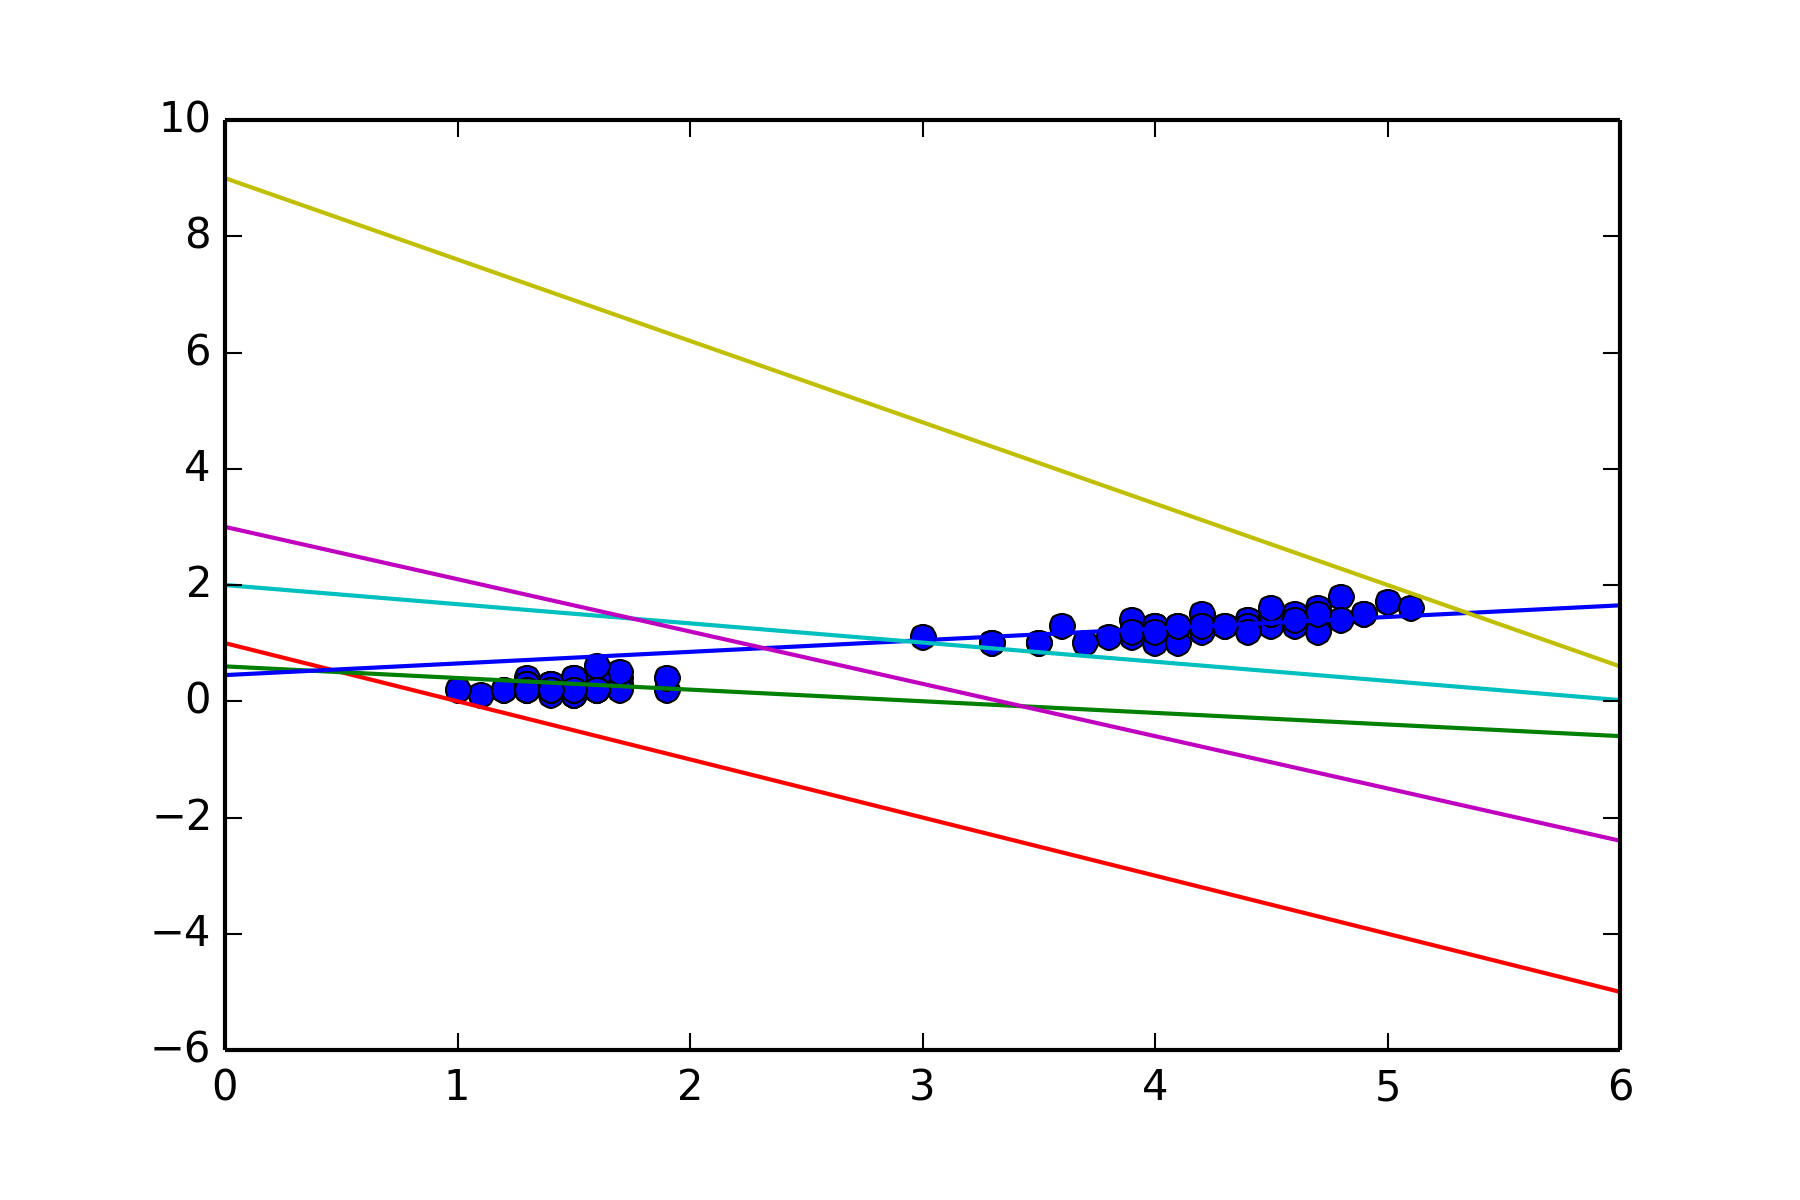
\includegraphics[width=0.7\linewidth]{graphics/gypothesis.png}
  \begin{tiny}
    \caption{Visualization of linearly separable \texttt{iris} dataset together with selected hypothesis.\label{fig:hyp}}
  \end{tiny}
  \vspace{1cm}
\end{figure}

\section{Algorithm design and tuning}
As suggested in~\citep{DBLP:journals/corr/GantiG13} we change our estimate of hypothesis uncertainty from the one presented in equation~\ref{eq:variance} to~\ref{eqn:expvar} given below.\\
\begin{equation}
\label{eqn:expvar}
U(\hat{L}_t(h)) = \frac{ \sqrt{ \log(t) } }
                       { 10 }
                  \sqrt{ V^\prime_t }
\end{equation}
$$
V^\prime_t = \left[
  \sum_{i = 1:n \text{~} \tau = 1:t} \frac{Q^\tau_i}{(p^\tau_i)^2} L^2(z(x_i))
  -
  \left( \sum_{\mathscr{Q}_t} L(z(x_i)) \right)^2
\right]_+
$$
This change is made solely to simplify and does not affect the variance estimate in any way.\\

With adjustment given above we implemented our solution in \texttt{Python} programming language(formatted as \texttt{iPython notebook}). We ran the experiment with different querying budgets: 1\%, 5\%, 10\%, 15\% and 20\% of initial dataset size. Figures~\ref{fig:conv} and~\ref{fig:conv.ALL} show change of risk mean estimate with number of queries made for listed above allowances.\\


\begin{figure}[htbp]
  \centering
  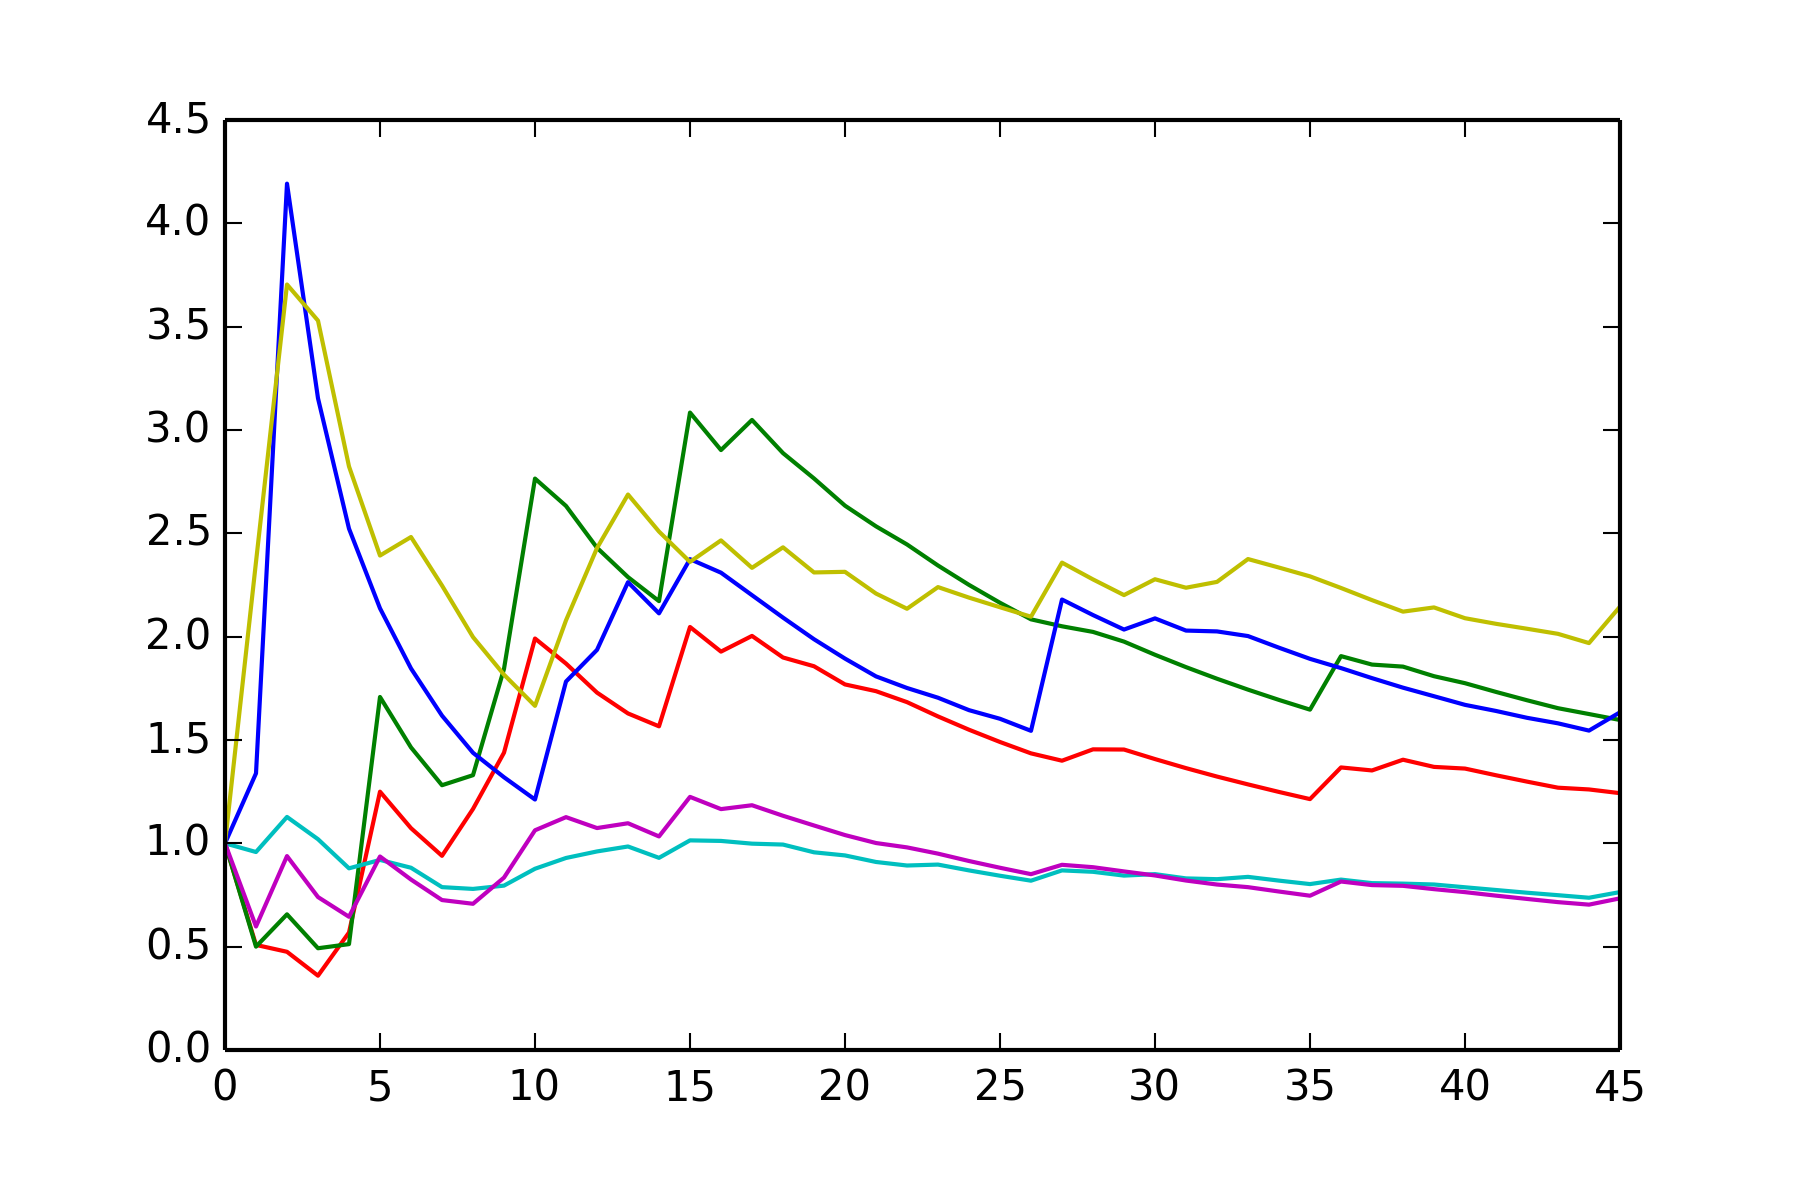
\includegraphics[width=0.7\linewidth]{graphics/convergence.png}
  \begin{tiny}
    \caption{Change of hypothesis risk estimation along time. Experiment conducted with query budget of 20\% of dataset size. Colours correspond to hypothesis shown in figure~\ref{fig:hyp}.\label{fig:conv}}
  \end{tiny}
  \vspace{1cm}
\end{figure}

\section{Results}
Figure~\ref{fig:conv} illustrates the results for the experiment with largest querying budget. The outcome is reasonable as it predicts \textcolor{magenta}{magenta} hypothesis as the best and \textcolor{cyan}{cyan} one as the second best; risk estimates for both these classifiers lie very close. Both these choices seems reasonable for given dataset---they make no error in classification.\\
\textcolor{green}{green} and \textcolor{blue}{blue} hypothesis also end up having close risk estimates and scoring 4\ts{th} and 5\ts{th} respectively. This result can be justified; the first one cuts one of the clouds in half, classifying approximately 75\% of exemplars correctly and the other hypothesis does the same with the other cloud of points.\\

\textcolor{red}{red} and \textcolor{Dandelion}{yellow} hypothesis classify all points correspondingly as $+$'s and $-$'s. The later one performs the worst what agrees with our prediction. On contrary the first one outperforms \textcolor{blue}{blue} and \textcolor{green}{green} what in this case should be treated as error; such behavior is possible and can be justified by algorithm querying more true negatives than positives.\\

We also present graphs for four other query budgets in figure~\ref{fig:conv.ALL}. In~\ref{fig:conv.ALL:01}(the smallest querying budget) the algorithm sent to oracle only 1 exemplar what yields random behavior. It seems like this particular point belonged to $+$ class placing \textcolor{blue}{blue} and \textcolor{Dandelion}{yellow} as the worst classifiers. Intuitively as \textcolor{Dandelion}{yellow} treats all exemplars as $-$'s, any query revealing $+$ point evaluates it as the worst hypothesis and any query resulting in $-$ point in the best; \textcolor{red}{red} hypothesis which was estimated as the best confirms preceding description.\\
Figure \ref{fig:conv.ALL:05}, corresponding to 5\% budget gives the correct answer by selecting \textcolor{magenta}{magenta} hypothesis. The second best prediction---\textcolor{cyan}{cyan}---is also correct, but the distance between these two optimal solutions an two sub-optimal, namely: \textcolor{red}{red} and \textcolor{green}{green}, seems to be really small. Due to this fact 5\% size oracle queries is still pron to severe errors.\\
Graph~\ref{fig:conv.ALL:10} provides good separation of optimal and sub-optimal hypothesis. Moreover, the predictions are still correct. For given dataset we can claim that 10\% sample is enough to give \emph{safe} prediction of the optimal hypothesis.\\
The following figure~\ref{fig:conv.ALL:15} improves the results given above by further separating optimal and sub-optimal answers. Experiment with 15\% sample in contrast to 10\% one estimates \textcolor{cyan}{cyan} hypothesis as the best and \textcolor{magenta}{magenta} one as the second best. Despite this phenomenon, all exemplars of dataset are classified correctly by chosen classifier. It seems that with more than one 0-error-rate hypothesis we need bigger number of oracle queries to choose the one with largest distance to both clouds of points. On the other hand \textcolor{cyan}{cyan} hypothesis might be better than \textcolor{magenta}{magenta} one in case we have not observed in our data any negative exemplar situated between two clouds due to the fact that they are rare.\\

Interesting fact can be observed by comparing \textcolor{red}{red} and \textcolor{Dandelion}{yellow} hypothesis through all experiments. As \textcolor{red}{red} is always predicted better than \textcolor{Dandelion}{yellow} our algorithm seems to send to oracle more points from top($+$) cloud than from the bottom($-$) one. This feature should be investigated further to better understand this phenomenon.\\

To sum up, for tested dataset 10\% sample seems to be the minimum we should use to ensure optimal hypothesis selection. All 0-error-rate hypothesis seems to have indistinguishable outcomes while querying less than 30\% of dataset volume. Finally, the behavior is quite reasonable and further studies should be carried out to examine properties of suggested solution.\\

\begin{figure}[htbp]
  \begin{subfigure}{.5\linewidth}\centering
    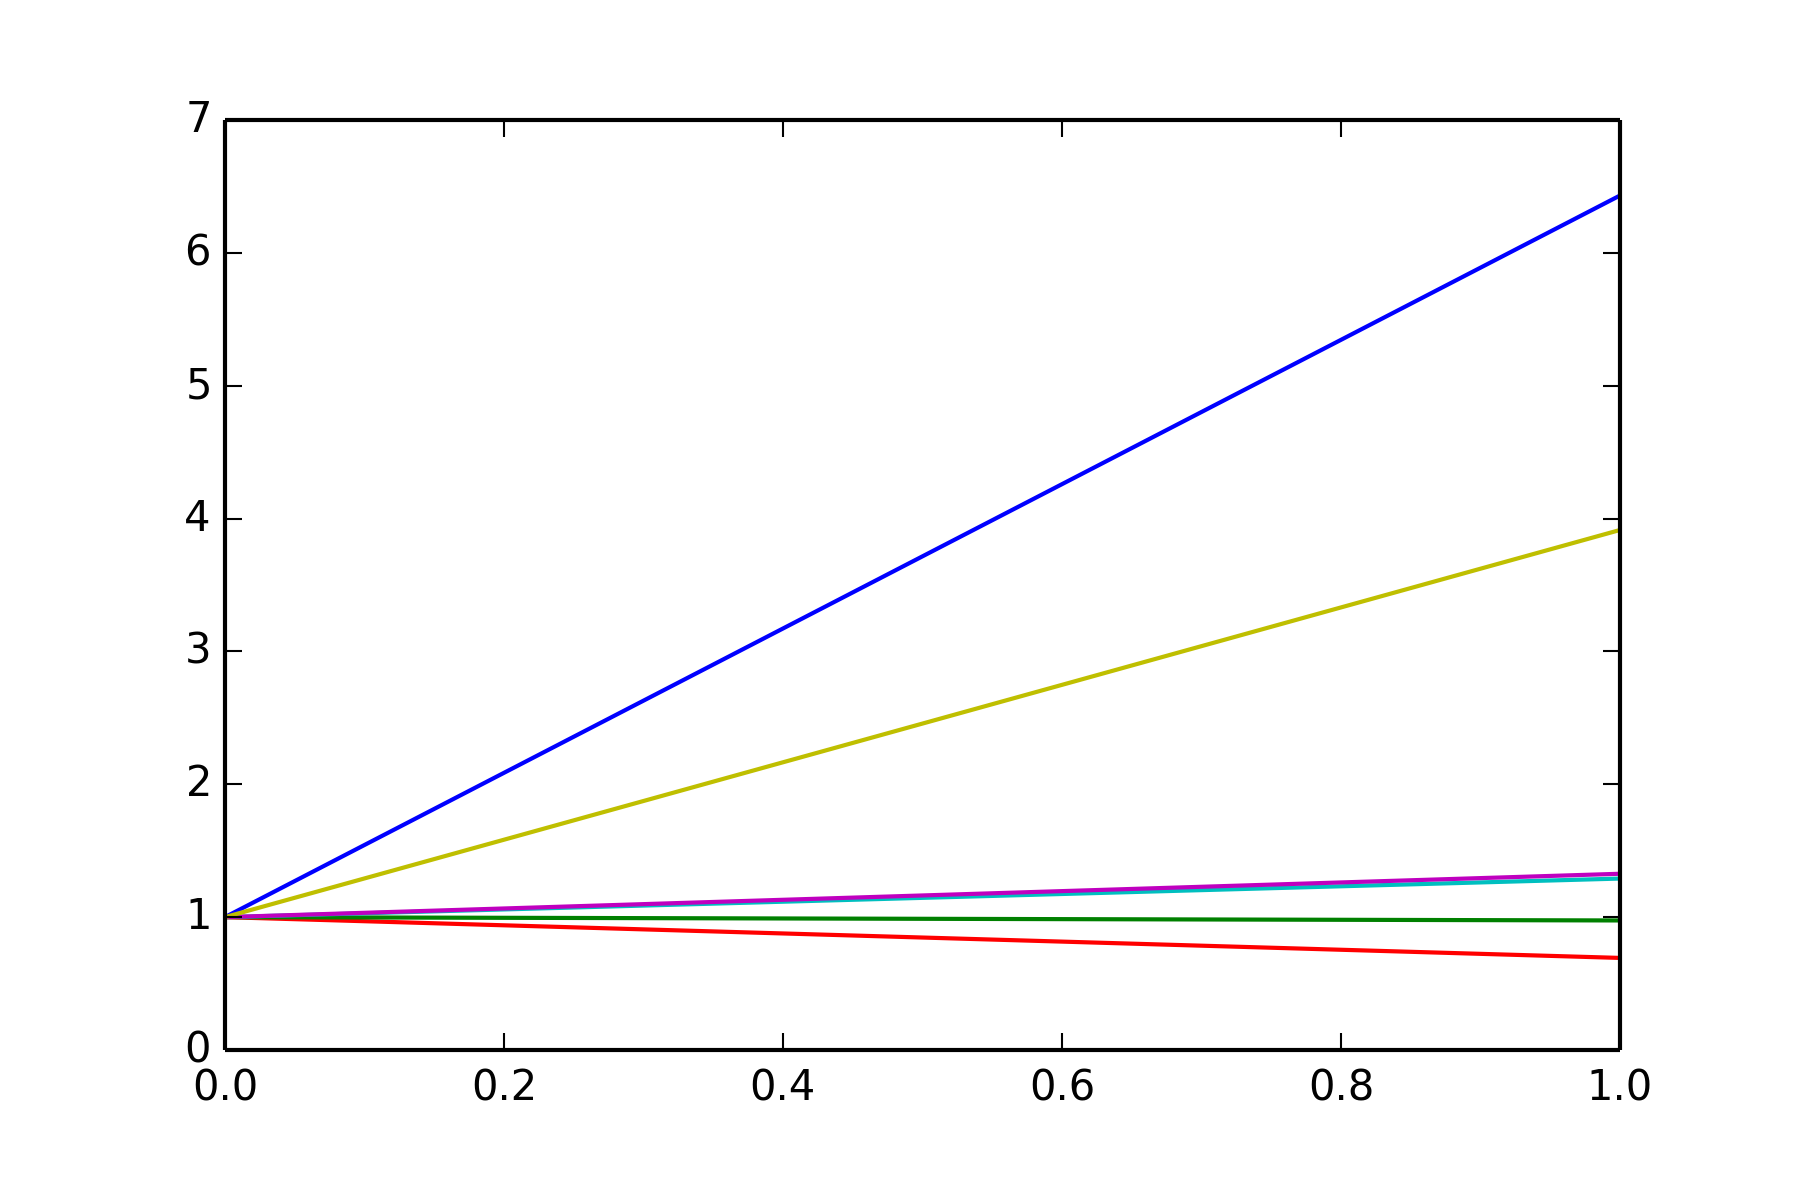
\includegraphics[width=1.1\textwidth]{graphics/convergence01.png}
    \caption{1\%\label{fig:conv.ALL:01}}
  \end{subfigure}
  \begin{subfigure}{.5\linewidth}\centering
    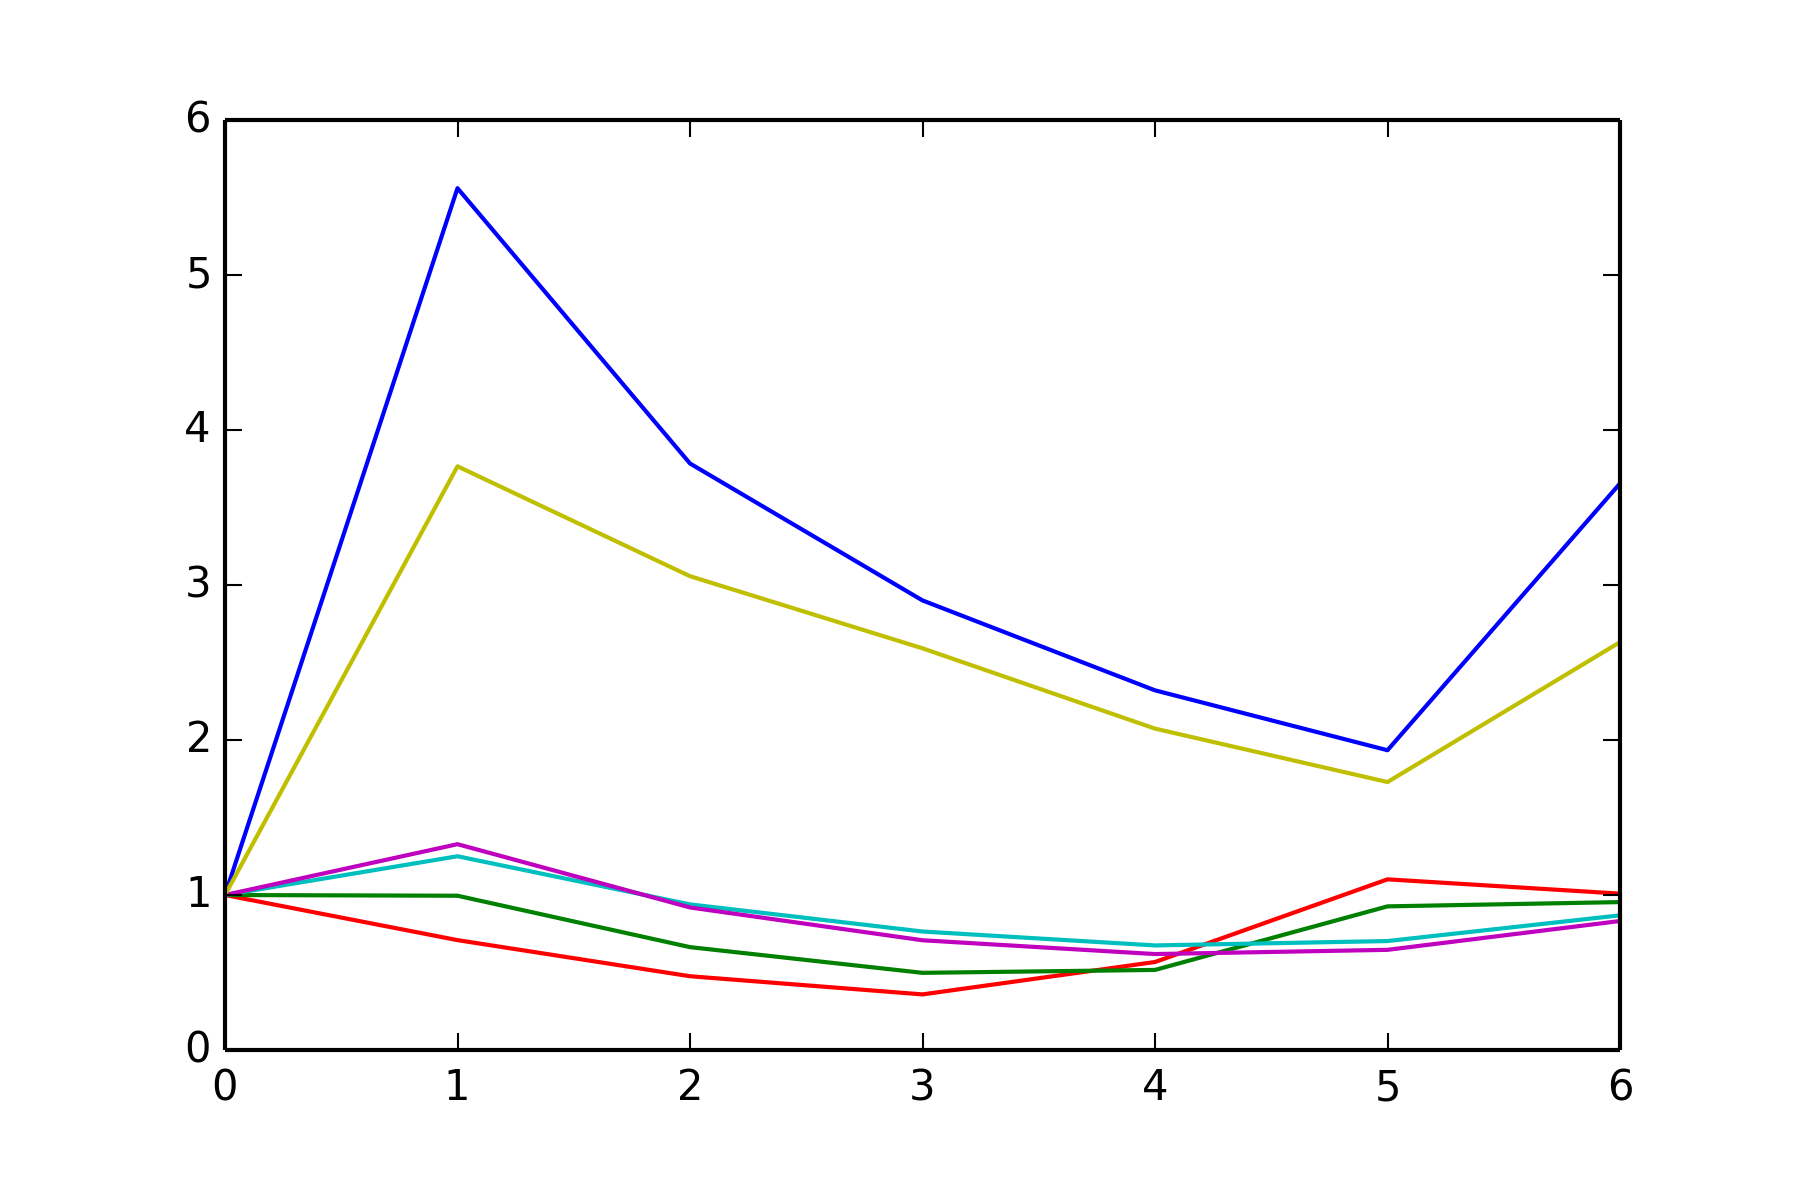
\includegraphics[width=1.1\textwidth]{graphics/convergence05.png}
    \caption{5\%\label{fig:conv.ALL:05}}
  \end{subfigure}\\[1ex]

    \begin{subfigure}{.5\linewidth}\centering
    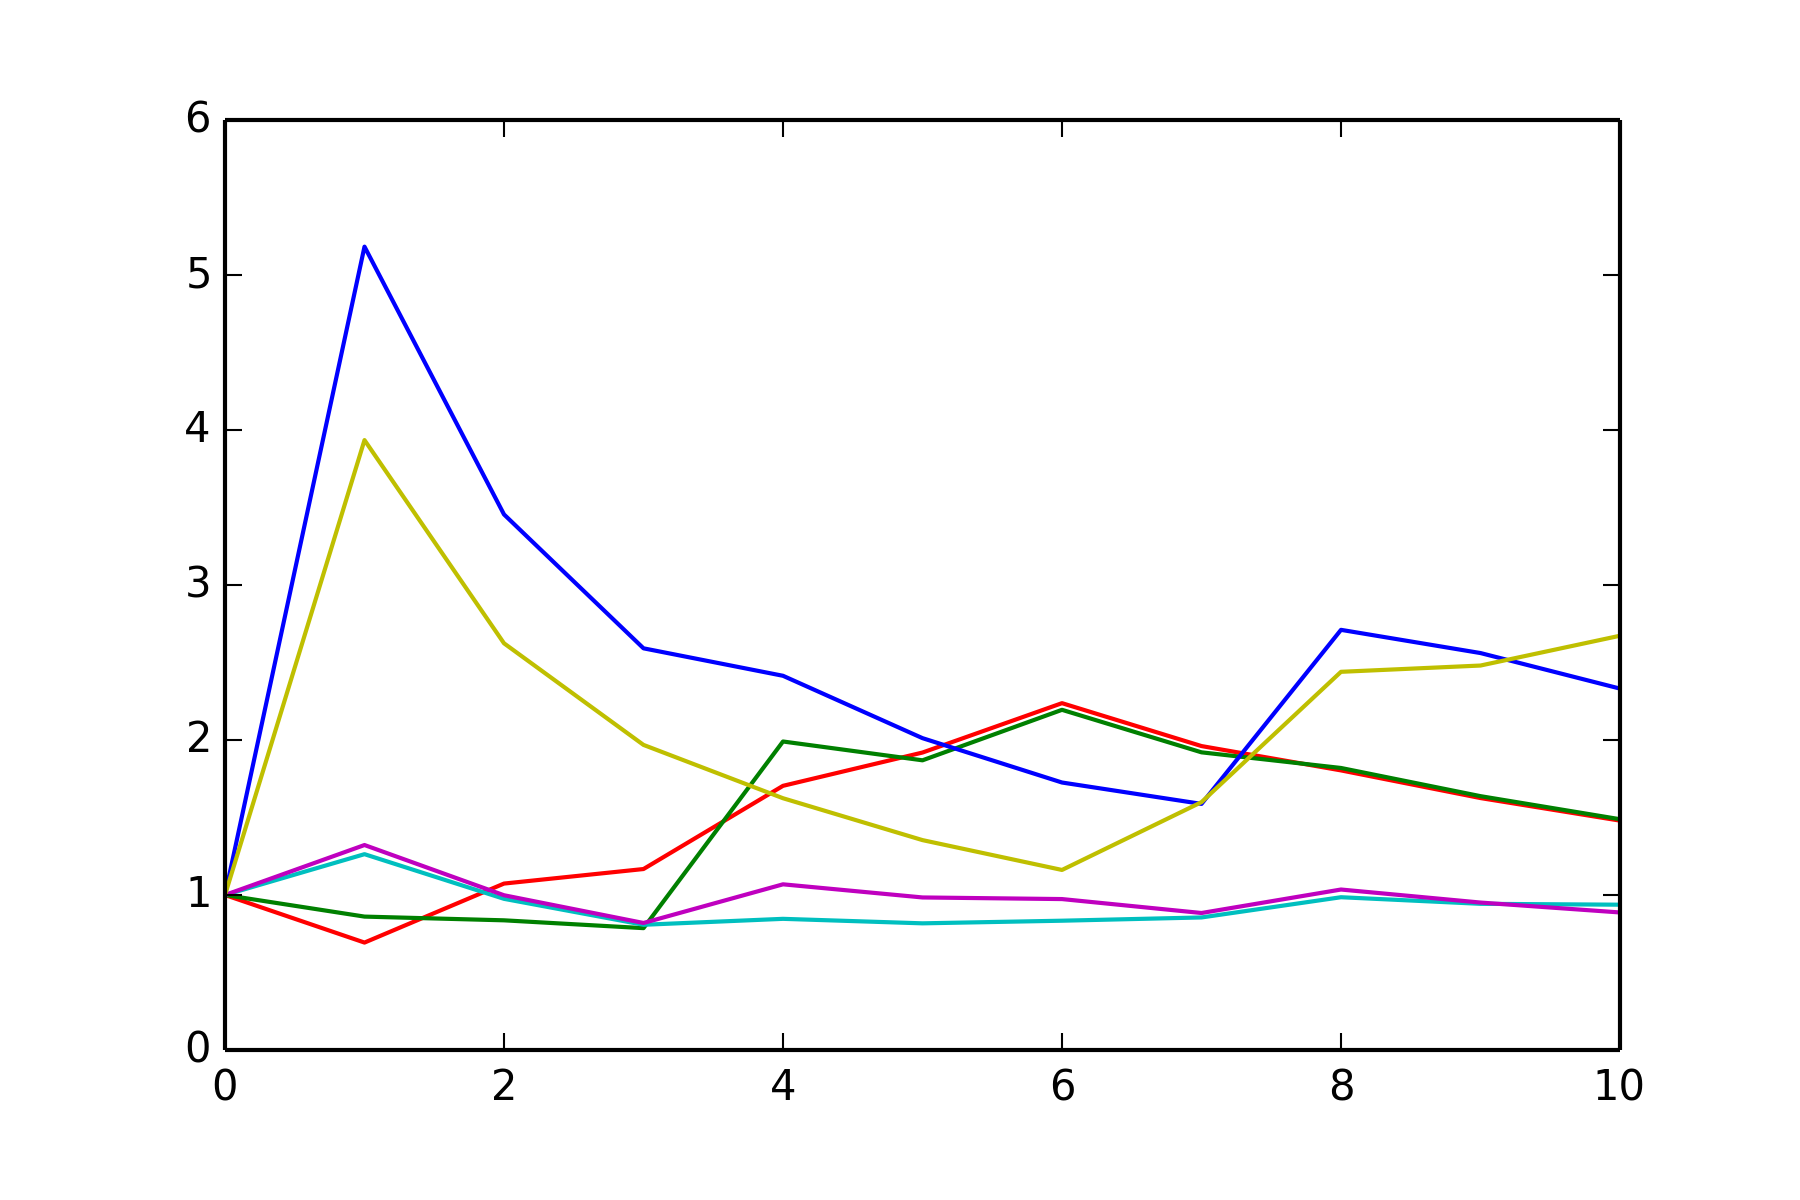
\includegraphics[width=1.1\textwidth]{graphics/convergence10.png}
    \caption{10\%\label{fig:conv.ALL:10}}
  \end{subfigure}
  \begin{subfigure}{.5\linewidth}\centering
    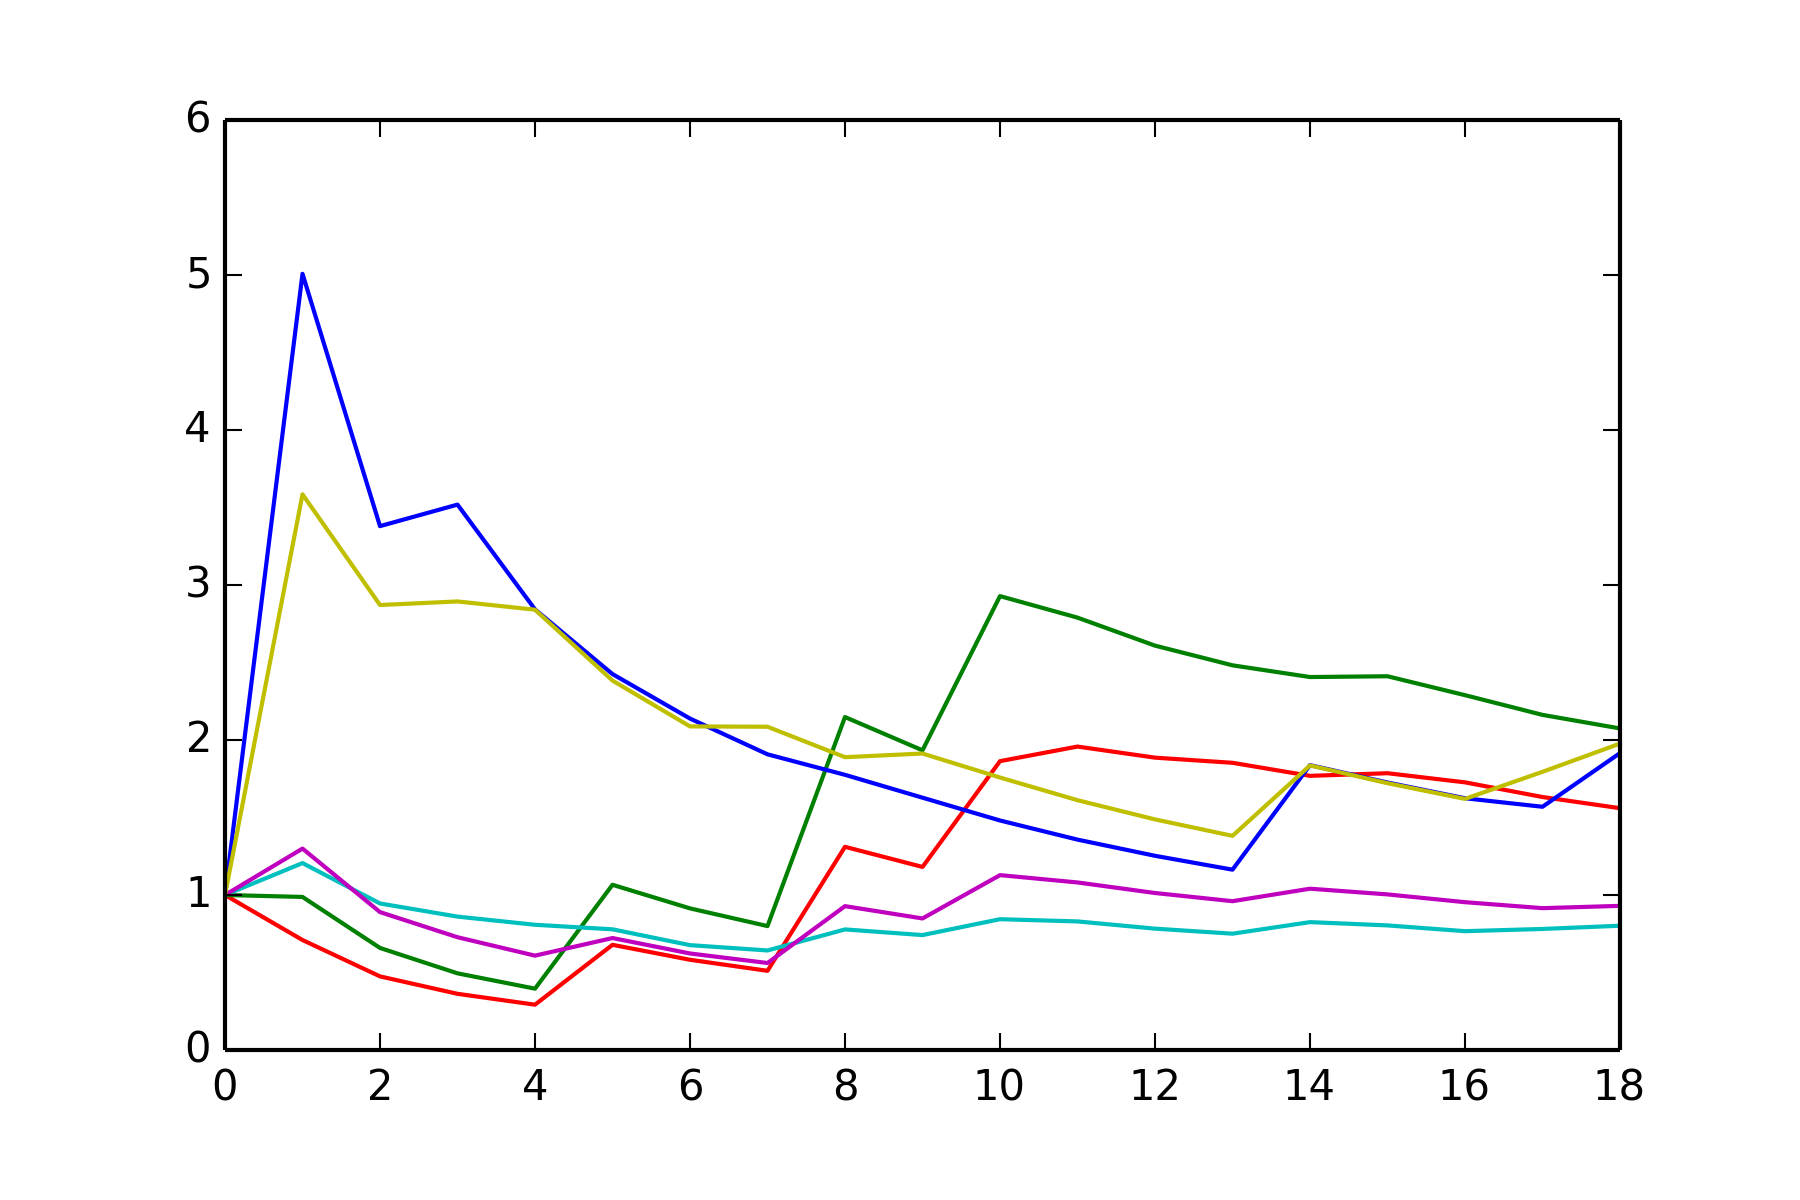
\includegraphics[width=1.1\textwidth]{graphics/convergence15.png}
    \caption{15\%\label{fig:conv.ALL:15}}
  \end{subfigure}

  \caption{Change of hypothesis risk estimation along time. Each sub-figure presents different percentage of oracle queries with regard to the number of points in the dataset. Colours correspond to hypothesis shown in figure~\ref{fig:hyp}.\label{fig:conv.ALL}}
\end{figure}


\section{LCB algorithm}

\begin{figure}[htbp]
  \centering
  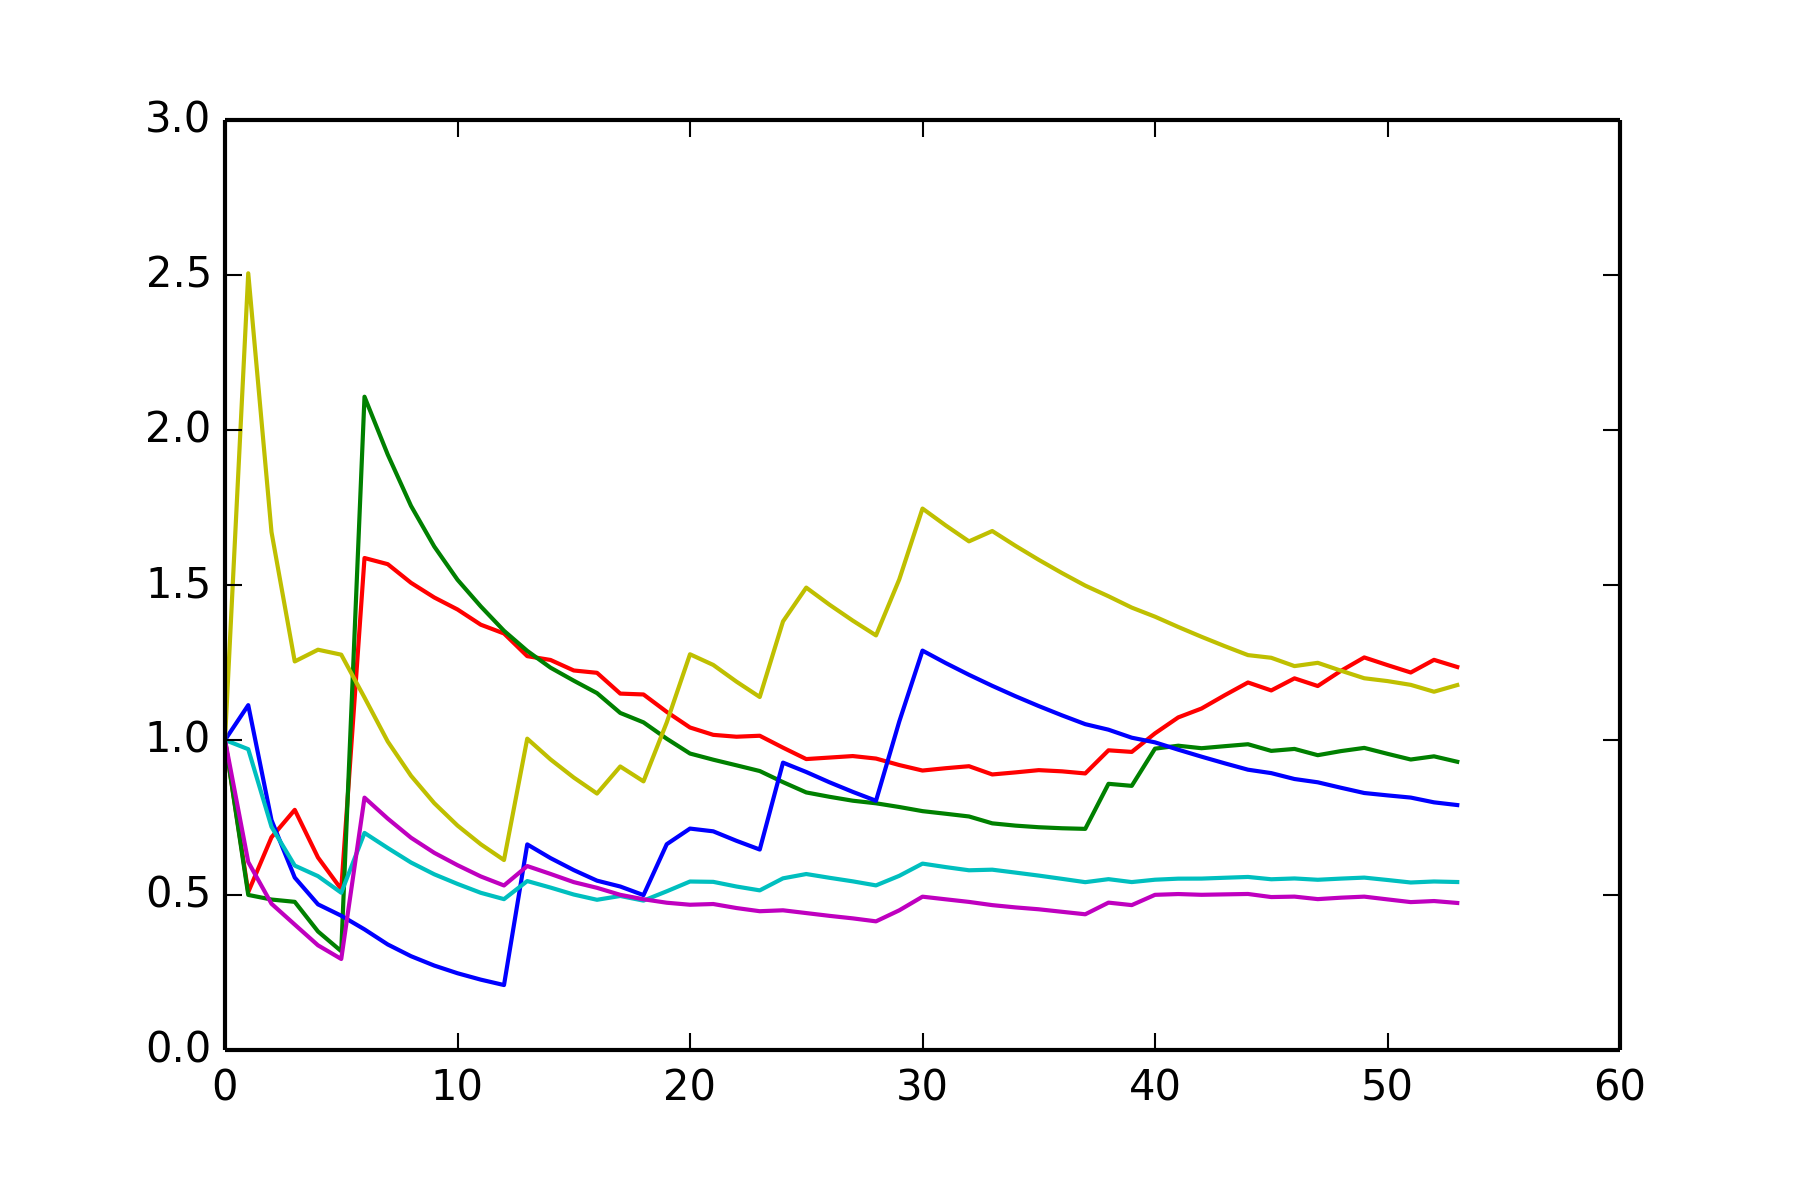
\includegraphics[width=0.7\linewidth]{graphics/convergence_LCB025.png}
  \begin{tiny}
    \caption{Change of hypothesis risk estimation along time with LCB selection mechanism. Experiment conducted with query budget of 20\% of dataset size. Colours correspond to hypothesis shown in figure~\ref{fig:hyp}.\label{fig:LCB_conv}}
  \end{tiny}
  \vspace{1cm}
\end{figure}

In this section we compare results achieved above for Thompson Sampling policy against ones achieved via \emph{Lower Confidence Bound} selection mechanism---straightforward application of algorithm~\ref{al:LCB-AL}. We conducted experiments for the same dataset and query budgets as above: 1\%, 5\%, 10\%, 15\% and 20\%.\\

The first striking feature of LCB while comparing to TS is higher number of queries made. LCB decides to ask already known points more often than TS.\\
For 20\% sample the LCB converges similarly to algorithm presented above. Optimal hypothesis is chosen at the end and it lies very close to the second optimal arm. Above optimal actions, we have two ``75\% correct'' hypothesis, and at the top(the worst) two arms which assigned to all exemplars singleton class. The only advantage of LCB over TS is \textcolor{red}{red} hypothesis being at the top rather than middle.\\
Here, same as above 1\% sample behaves randomly and does not contain any informative content.\\
The 5\% experiment also groups the answers into three pairs: \textcolor{blue}{blue}--\textcolor{Dandelion}{yellow}, \textcolor{cyan}{cyan}--\textcolor{magenta}{magenta}, \textcolor{green}{green}--\textcolor{red}{red} like in 20\% case. Here, the two 0-error-rate answers are predicted as sub-optimal in contrast to correct prediction in TS.\\
10\% case yields similar behavior to corresponding experiment with TS approach. It does a bit worse as \textcolor{green}{green} hypothesis over-performs \textcolor{cyan}{cyan}---which is one of optimal hypothesis. Despite, this fact the the best---\textcolor{magenta}{magenta}---hypothesis is chosen.\\
Finally, 15\% results in similar randomness of sub-optimal arms as corresponding TS trial. Nevertheless, two optimal hypothesis are indicated as the best with fine distance to all the other actions.\\

To sum up, two approaches result in similar behavior. The best hypothesis converges the same in both cases; sub-optimal ones also follow comparable paths with a bit of randomness. While comparing both methods with results shown above we cannot unambiguously say which algorithm performs better. We plan to conduct additional experiments in the near future to address this uncertainty.\\


\begin{figure}[htbp]
  \begin{subfigure}{.5\linewidth}\centering
    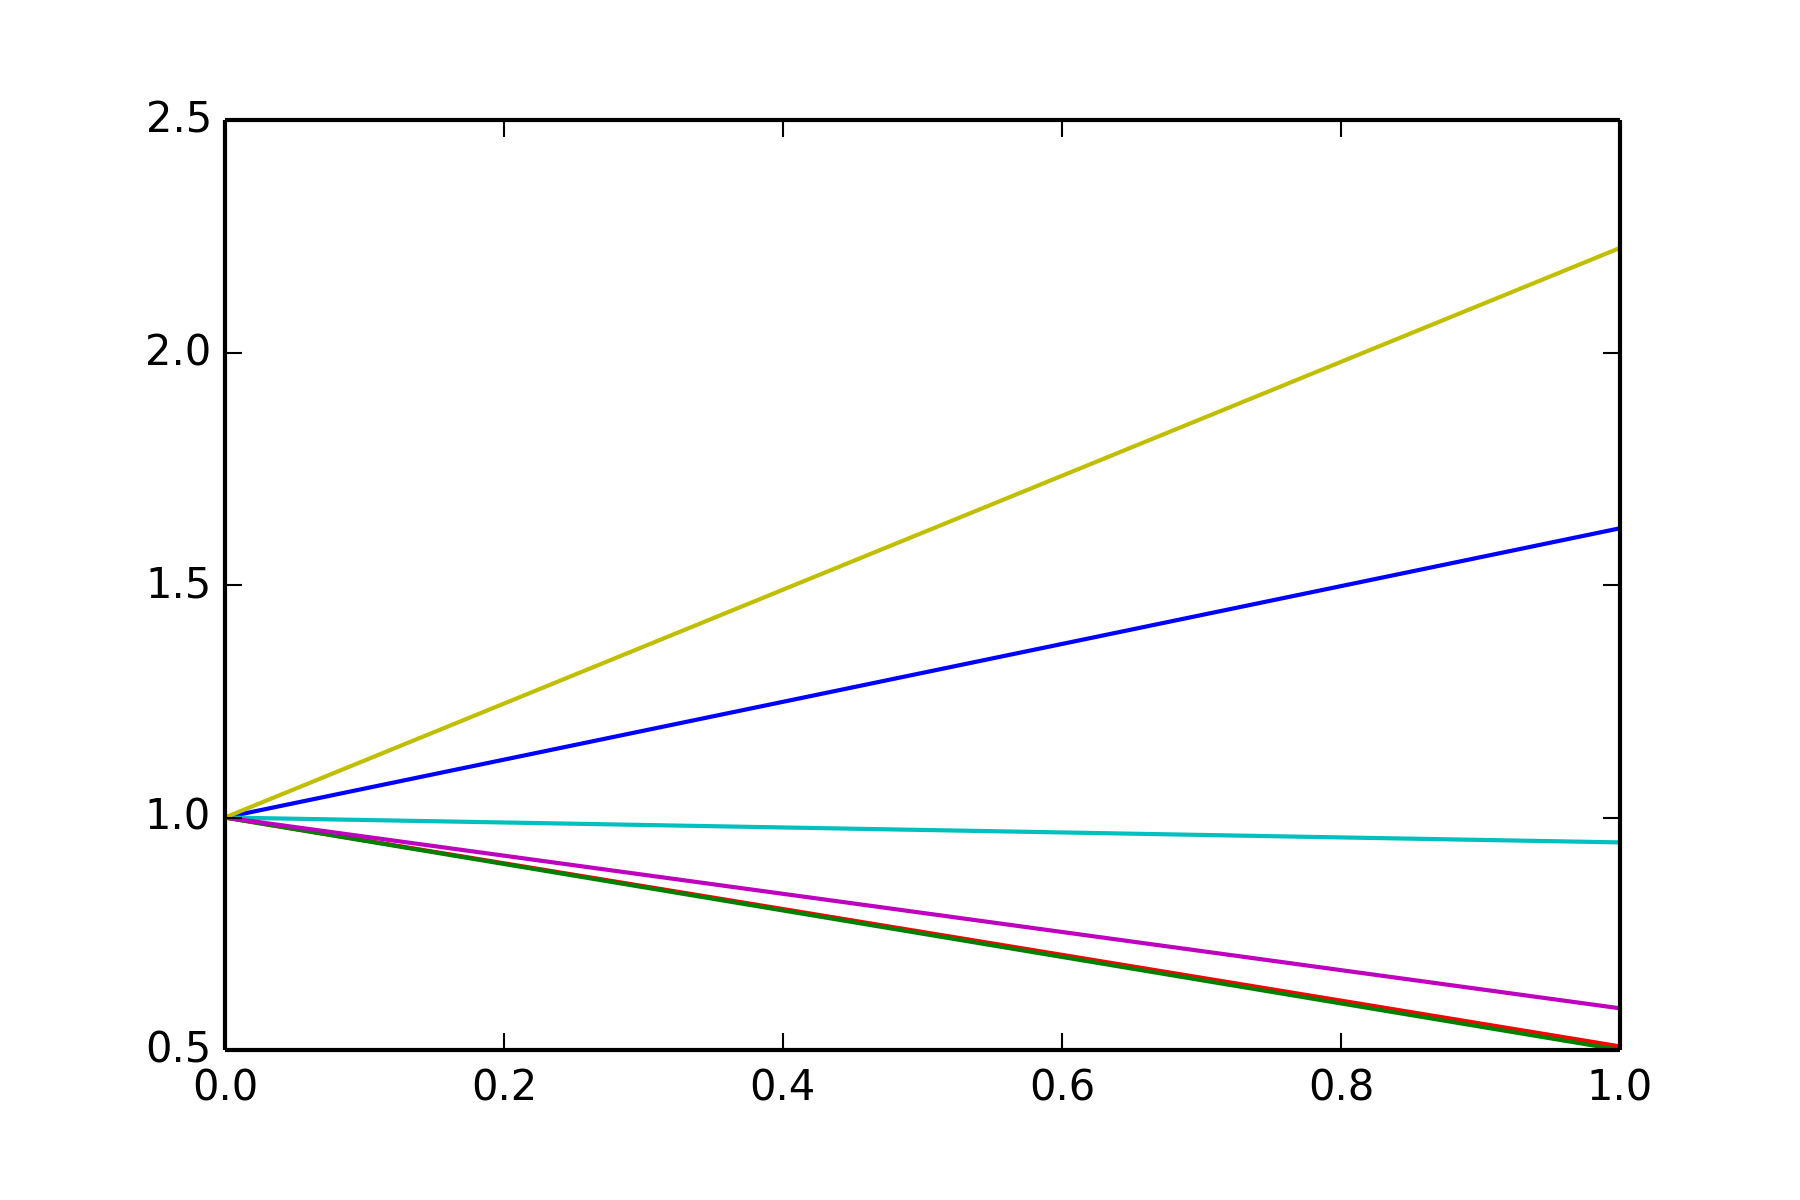
\includegraphics[width=1.1\textwidth]{graphics/convergence_LCB001.png}
    \caption{1\%\label{fig:LCB_conv.ALL:01}}
  \end{subfigure}
  \begin{subfigure}{.5\linewidth}\centering
    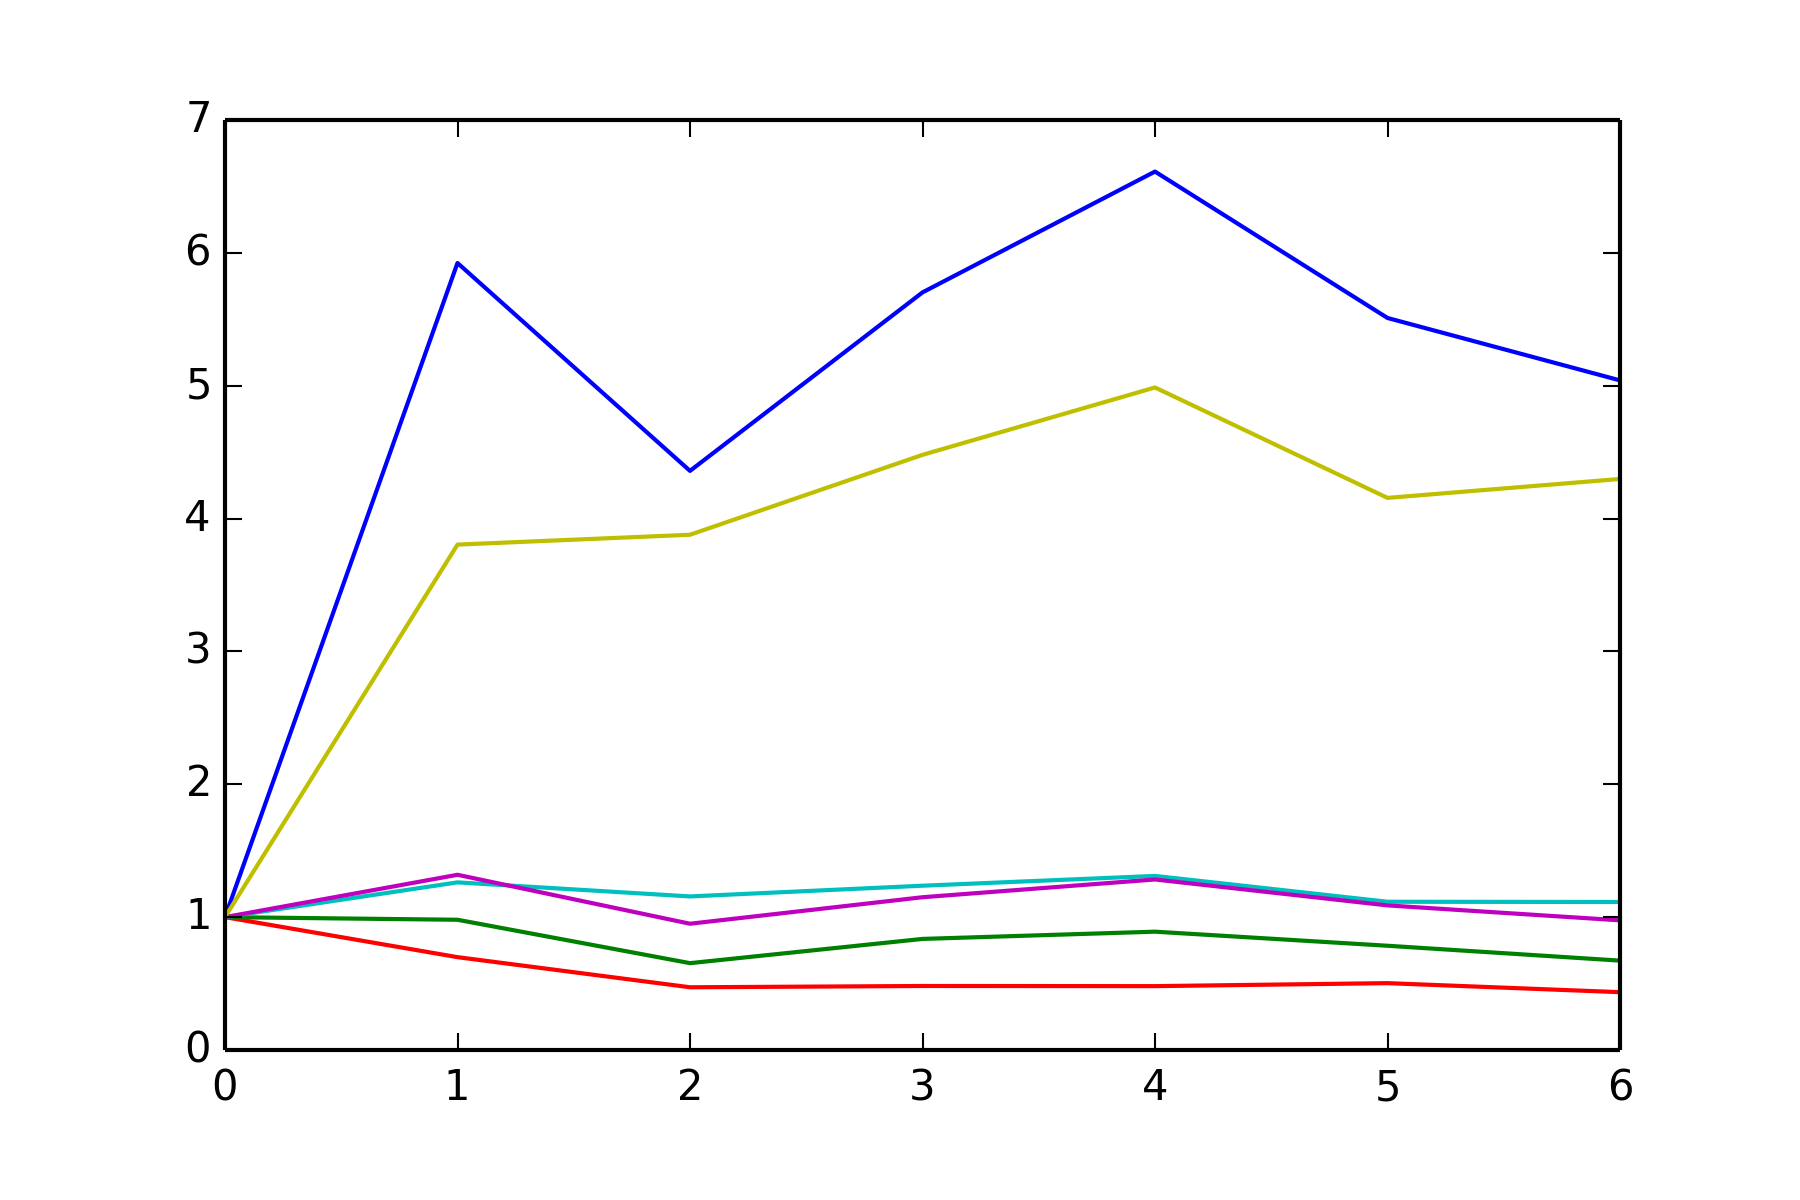
\includegraphics[width=1.1\textwidth]{graphics/convergence_LCB005.png}
    \caption{5\%\label{fig:LCB_conv.ALL:05}}
  \end{subfigure}\\[1ex]

    \begin{subfigure}{.5\linewidth}\centering
    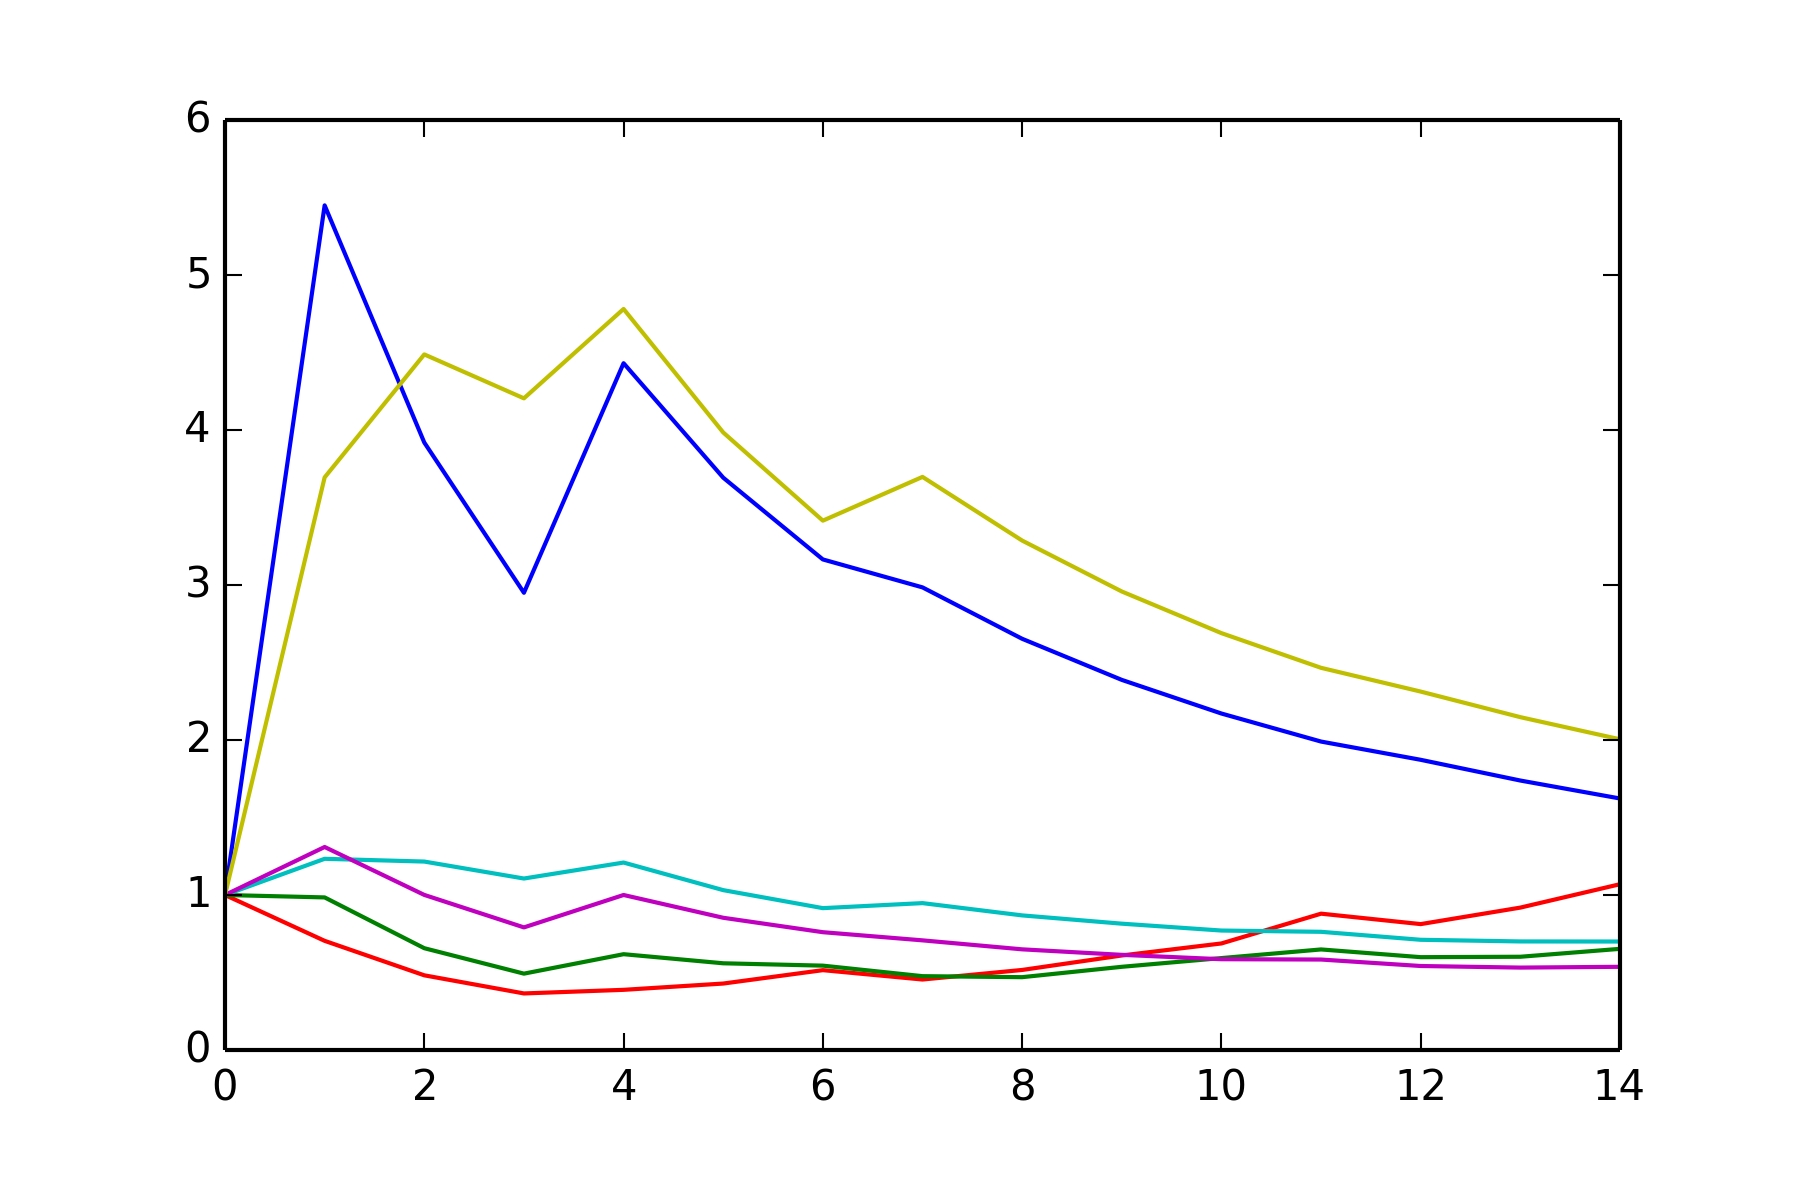
\includegraphics[width=1.1\textwidth]{graphics/convergence_LCB010.png}
    \caption{10\%\label{fig:LCB_conv.ALL:10}}
  \end{subfigure}
  \begin{subfigure}{.5\linewidth}\centering
    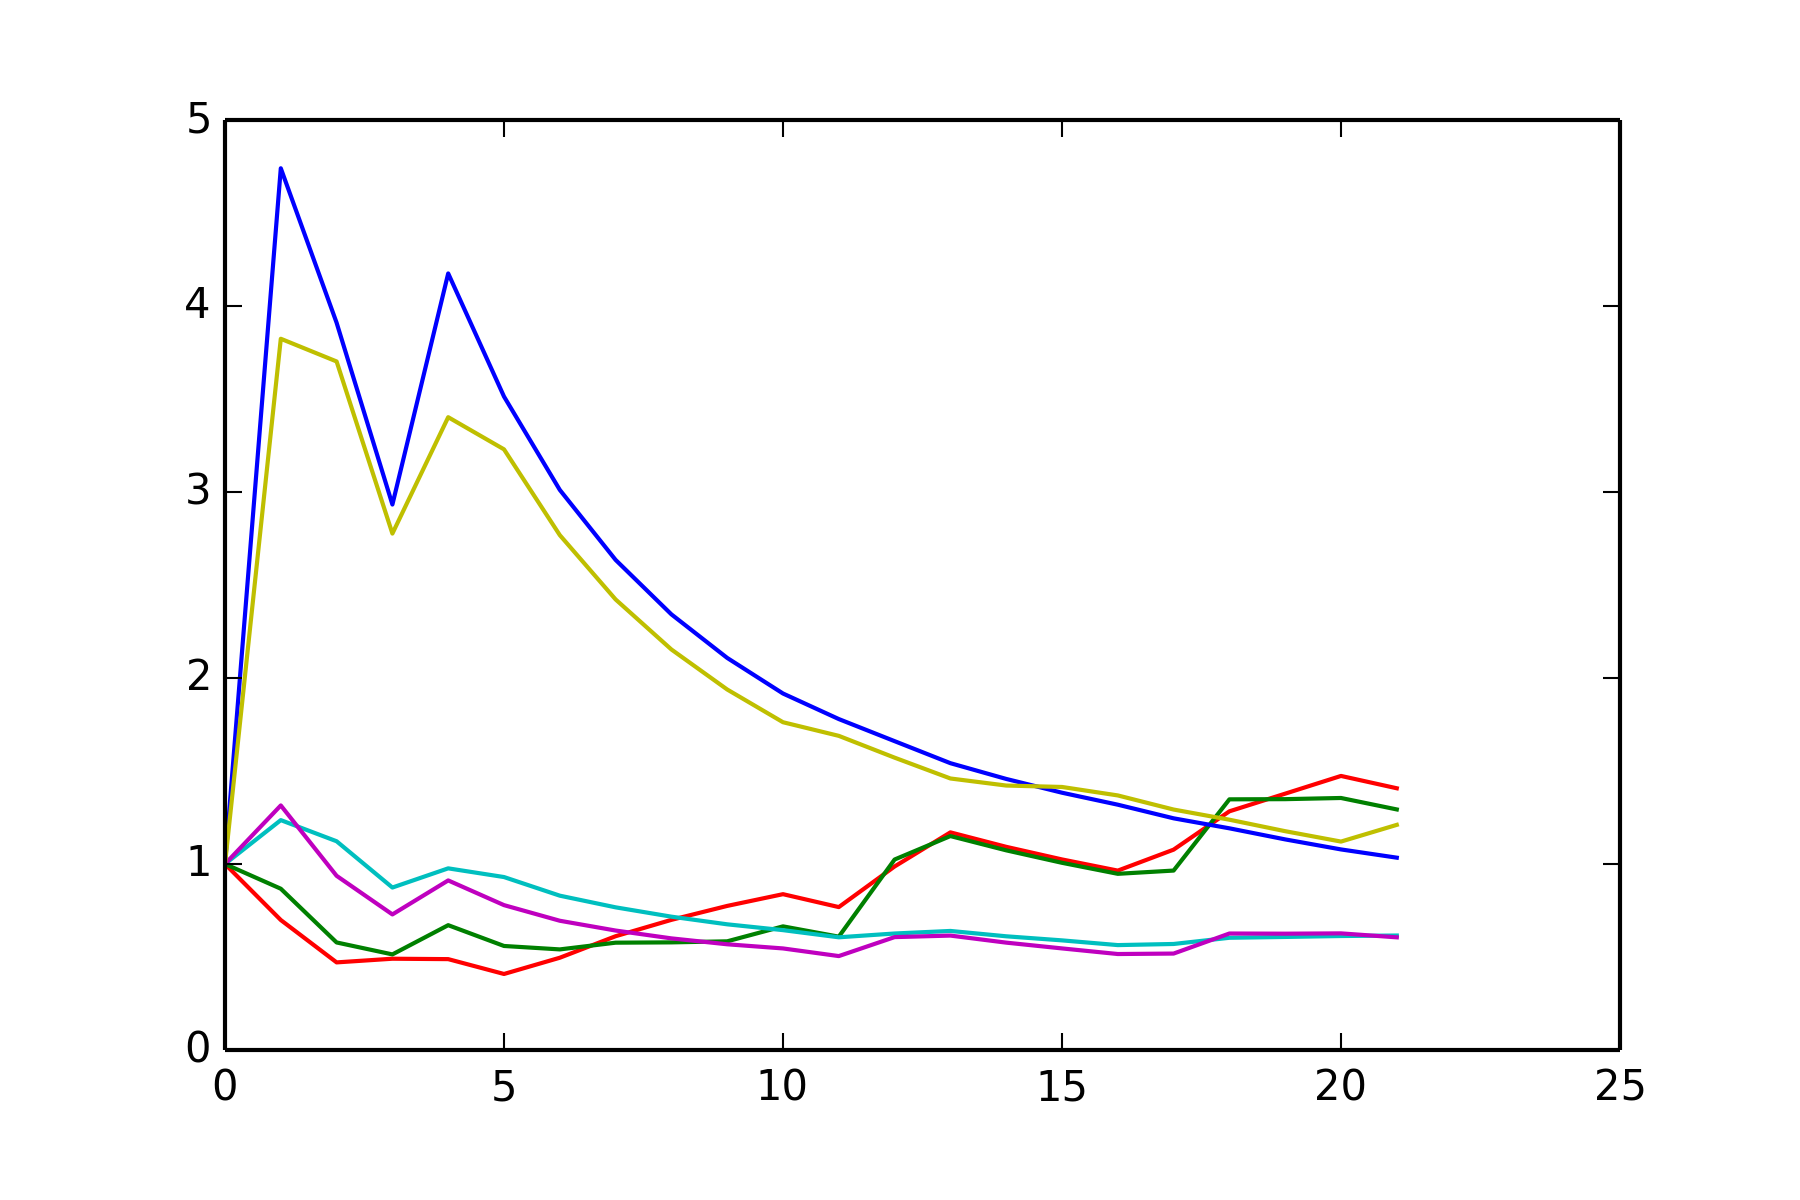
\includegraphics[width=1.1\textwidth]{graphics/convergence_LCB015.png}
    \caption{15\%\label{fig:LCB_conv.ALL:15}}
  \end{subfigure}

  \caption{Change of hypothesis risk estimation along time with LCB selection mechanism. Each sub-figure presents different percentage of oracle queries with regard to the number of points in the dataset. Colours correspond to hypothesis shown in figure~\ref{fig:hyp}.\label{fig:LCB_conv.ALL}}
\end{figure}




\section{Tweaks, Alternatives and Improvements\label{sec:qimprove}}
Presented in section~\ref{sec:thompsonimprovement} solution uses estimate of risk of given hypothesis and value representing uncertainty about this estimate. Both these quantities are updated after each oracle query is done. We can change this process by assuming uniform prior over all hypothesis and updating the distributions by Bayes rule when new information is revealed---a point is queried.\\
This method would demand posterior to estimate fit of given hypothesis for both known and unknown data. Queried point would either support hypothesis by agreeing with it's predictions or discourage this choice by not agreeing.\\
The point to query would be chosen based on being the most informative for current hypothesis. For instance point laying closest to boundary---having largest contribution to variance estimate.\\


Another possible improvement can be used to significantly reduce hypothesis space to the ones that are most probable a good fit. It can be acquired by first doing unsupervised learning on dataset(clustering, U-SVM) with number of threshold parameters to produce range of linear classifiers. The output of such process can be incorporated as a subset of our hypothesis space.\\


\section{Lookahead}
Presented here work covers brief introduction to multi-armed bandits world with stress put on Thompson sampling approach. It also deeply explains possible application of MAB in machine learning---active learning---by presenting one of its kind~\citep{DBLP:journals/corr/GantiG13} work. We took a step ahead by proposing Thompson approach to the problem by replacing lower confidence bound method chosen by authors with Thompson Sampling inspired hypothesis selection mechanism. Finally we planned, coded and carried out the experiment to examine results of our methodological change in algorithm. The outcomes seems promising and vouch for our intuition behind the active learning problem.\\

Due to time constrains, we were not able to improve our Thompson approach as described above(\S\ref{sec:qimprove}). We also could not perform full range of tests and comparisons between already existing algorithms and proposed one. We hope do address these issues in the near future.\\

Finally, we think that our algorithm along with simplicity brings low computational costs and performance comparable with other available solutions. We consider presented here algorithm to bring a good framework for active leaning problems in machine learning world in near future.\\

\begin{center}
\noindent \line(1,0){250}
\end{center}



\bibliography{ref}{}
% \bibliographystyle{plain}
\bibliographystyle{plainnat}



% \newpage
% \begin{center}~\\[10cm] \textbf{\huge FIN} \end{center}


% \appendix
% \chapter{Code snippets}

% \label{snip:normaldist}PDF of normal distribution with mean $0$ and standard deviation $5$.
% \begin{lstlisting}
% x   <- seq(-30,30,length=10000)
% y   <- dnorm(x,mean=0, sd=5)
% plot(x,y, type="l", lwd=1)
% \end{lstlisting}

% \label{snip:thompsonsampling}Creating multiple normal distributions to visualize Thompson sampling.
% \begin{lstlisting}
%  x   <- seq(5,15,length=1000)
%  y   <- dnorm(x,mean=10, sd=30)
% plot(x,y, type="l", lwd=1)
% sam <- sample(x, 10)
% points(sam,dnorm(sam, 10, 1), col="green")

% # for a few distributions
% \end{lstlisting}

\end{document}
